\documentclass[11pt,
			   %10pt, 
               %hyperref={colorlinks},
               aspectratio=169,
               hyperref={colorlinks}
               ]{beamer}
\usetheme{Singapore}
\usecolortheme[snowy, cautious]{owl}

\usepackage[utf8]{inputenc}
\usepackage[T1]{fontenc}
\usepackage[american]{babel}
\usepackage{graphicx}
\usepackage{hyperref}

\hypersetup{
    colorlinks=true,
    urlcolor=[rgb]{0,0,0.61},
    linkcolor=[rgb]{0,0,0.61}}
\definecolor{magenta}{RGB}{255, 0, 255}

\usepackage[natbib=true,style=numeric,backend=bibtex,useprefix=true]{biblatex}

\definecolor{OwlGreen}{RGB}{51,0,102} % easier to see
\setbeamertemplate{bibliography item}{\insertbiblabel}
\setbeamerfont{caption}{size=\footnotesize}
\setbeamertemplate{frametitle continuation}{}

\setcounter{tocdepth}{1}
\renewcommand*{\bibfont}{\scriptsize}
\addbibresource{lecture_5.bib}

\renewcommand*{\thefootnote}{\fnsymbol{footnote}}

\usenavigationsymbolstemplate{}
\setbeamertemplate{footline}{%
    \raisebox{5pt}{\makebox{\hfill\makebox[20pt]{\color{gray}
          \scriptsize\insertframenumber}}}\hspace*{5pt}}
          
          
%-------------------------------------------------------------------------------

\usepackage{epigraph}
\setlength\epigraphwidth{14cm}
\setlength\epigraphrule{0pt}
\usepackage{etoolbox}
\makeatletter
\patchcmd{\epigraph}{\@epitext{#1}}{\itshape\@epitext{#1}}{}{}
\makeatother

%--------------------------------------------------------------------------------------------
          
\author{Patrick Hall}
\title{Responsible Machine Learning\footnote{\tiny{This material is shared under a \href{https://creativecommons.org/licenses/by/4.0/deed.ast}{CC By 4.0 license} which allows for editing and redistribution, even for commercial purposes. However, any derivative work should attribute the author.}}}
\subtitle{Lecture 5: Machine Learning Model Debugging}
\institute{The George Washington University}
\date{\today}


\begin{document}
	
	\maketitle
	
	\begin{frame}
	
		\frametitle{Contents}
		
		\tableofcontents{}
		
	\end{frame}
	
	
%-------------------------------------------------------------------------------
	\section{Overview}
%-------------------------------------------------------------------------------

		\subsection*{} %just for progress indicator
			
		\begin{frame}
		
			\frametitle{A Responsible Machine Learning Workflow\footnote{\href{https://www.mdpi.com/2078-2489/11/3/137/htm}{\textit{A Responsible Machine Learning Workflow}}}}
			
			\begin{figure}[htb]
				\begin{center}
					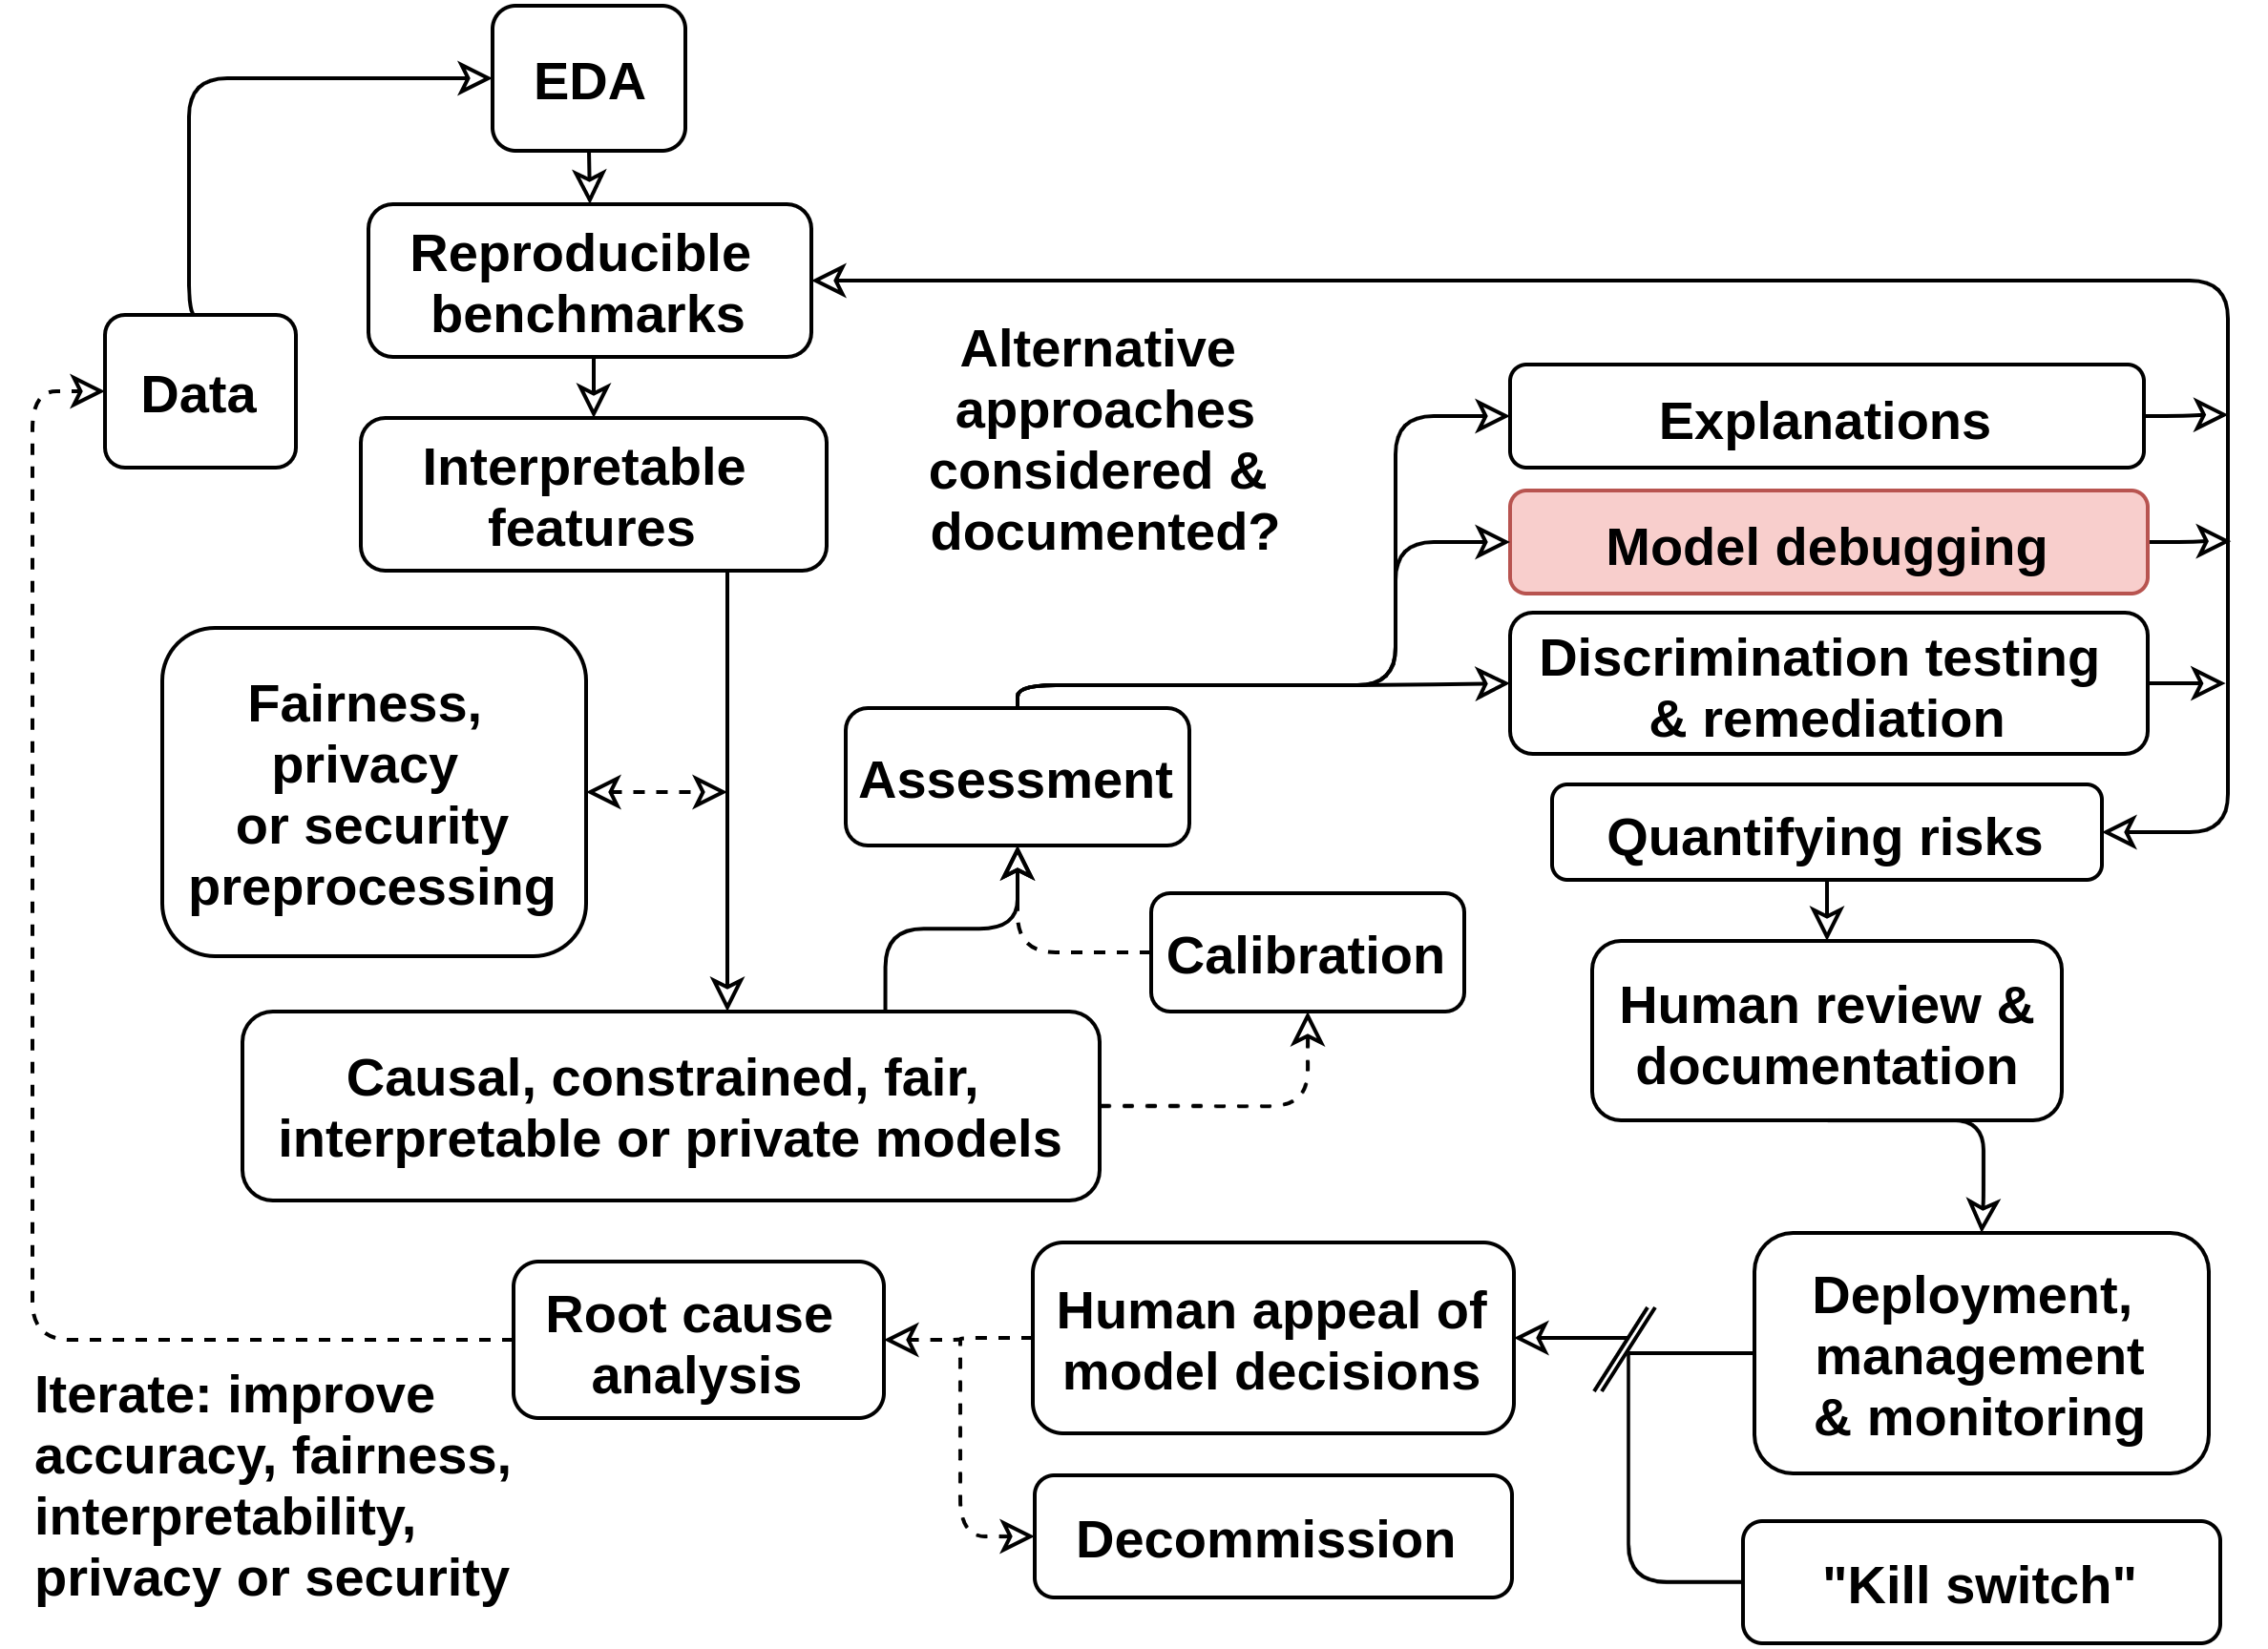
\includegraphics[height=150pt]{../img/rml_diagram_lec4_hilite.png}
					\label{fig:blueprint}
				\end{center}
			\end{figure}		
					
		\end{frame}	

		\begin{frame}
		
			\frametitle{What is Model Debugging?}
		
			\begin{itemize}
				\item Model debugging is an emergent discipline focused on discovering and remediating errors in the internal mechanisms and outputs of machine learning models.\footnote{\tiny{See \url{https://debug-ml-iclr2019.github.io/} for numerous model debugging approaches.}} 
				\item Model debugging attempts to test machine learning models like code (because the models are code).
				\item Model debugging promotes trust directly and enhances interpretability as a side-effect.
				\item Model debugging is similar to regression diagnostics, but for nonlinear machine learning models.
			\end{itemize}
		
		\end{frame}

	
		\begin{frame}[t]

 				\frametitle{Trust and Understanding}
      
 				\begin{figure}
   				\begin{center}
     					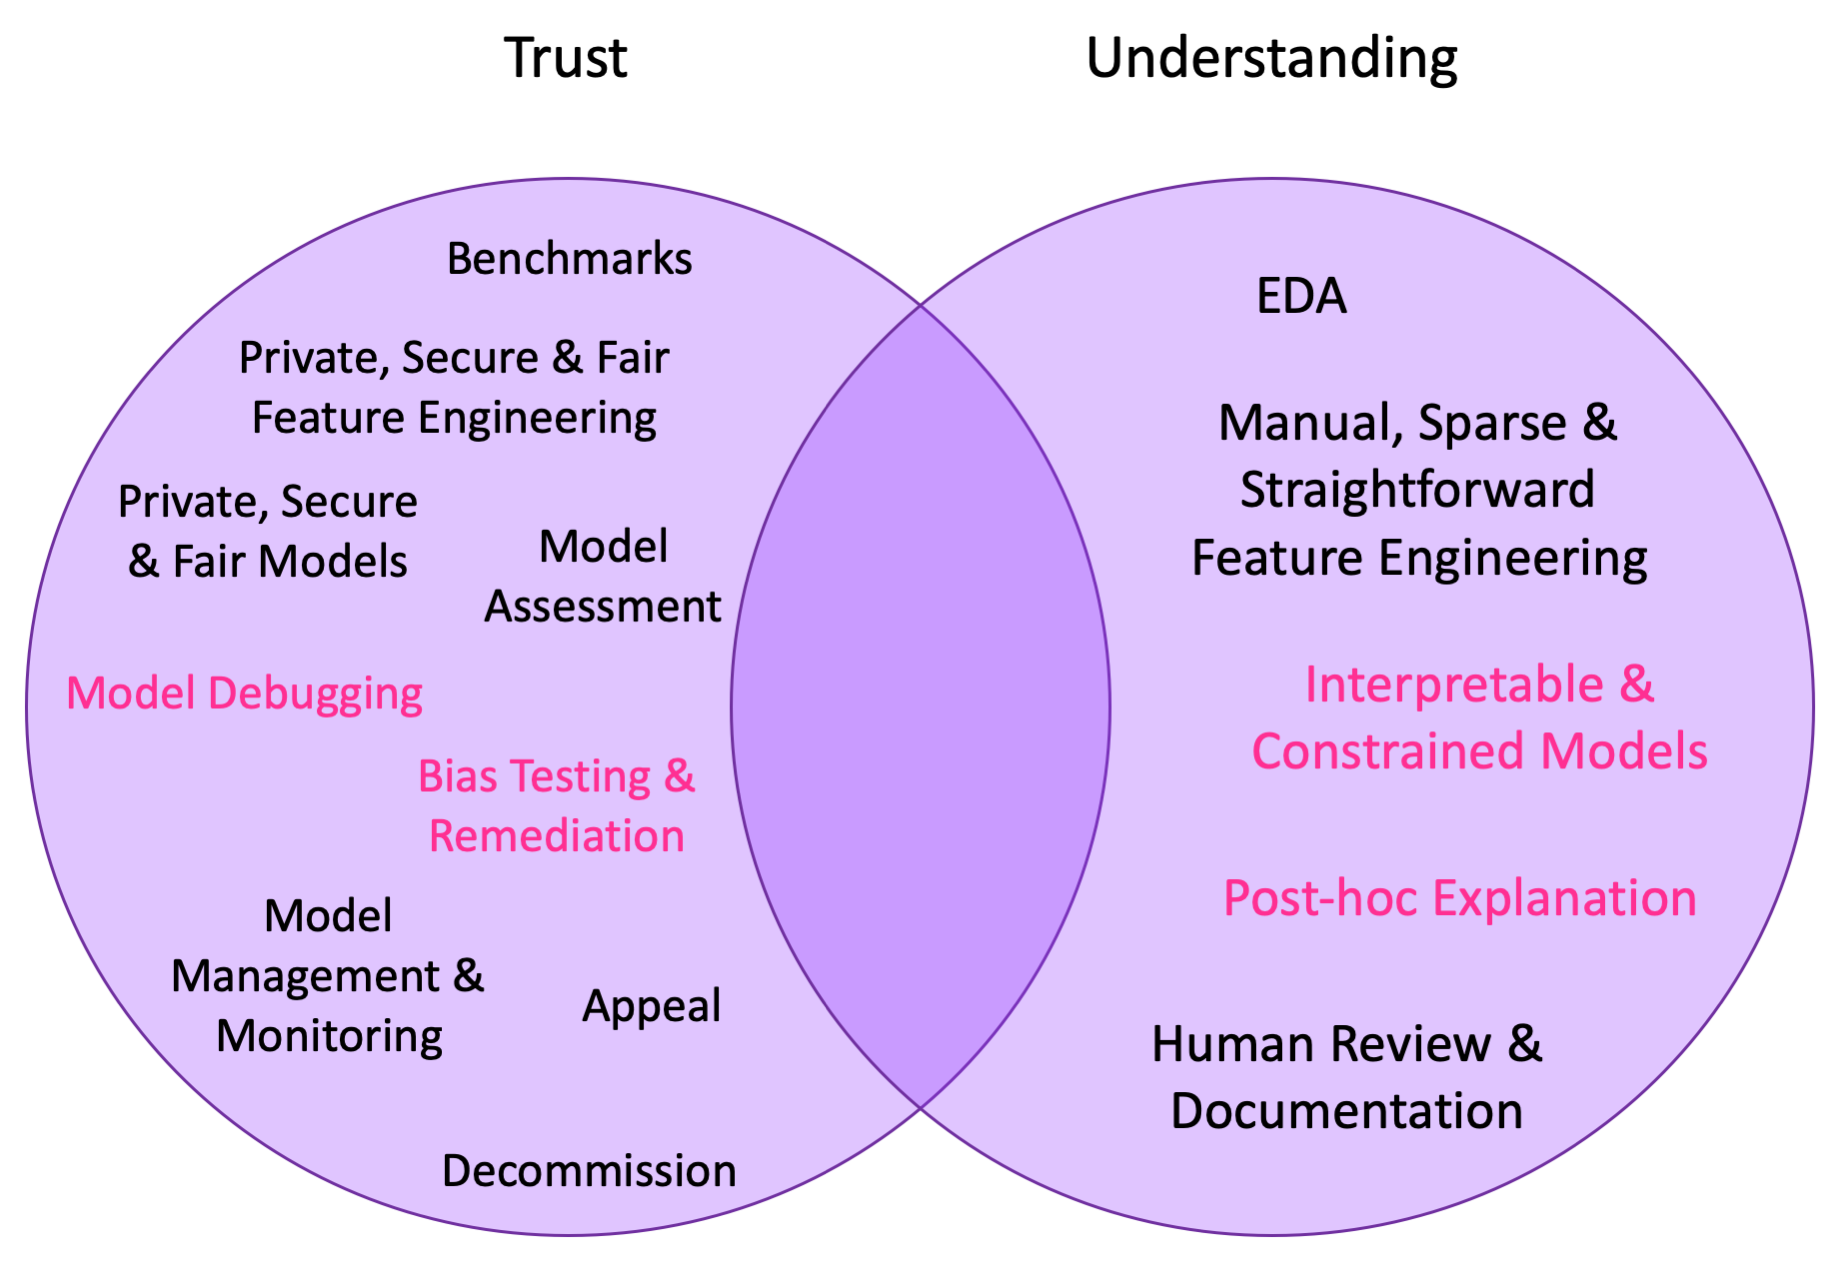
\includegraphics[height=130pt]{../img/trust_understanding.png}
   				\end{center}
 				\end{figure}

 			Trust and understanding in machine learning are different but complementary goals, and they are technically feasible \textit{today}.
    
		\end{frame}

%-------------------------------------------------------------------------------
	\section{Why Debug}
%-------------------------------------------------------------------------------

%-------------------------------------------------------------------------------
		\subsection*{}
%-------------------------------------------------------------------------------	

			\begin{frame}
				
				\frametitle{Reminder: What is Machine Learning?}
				
					\begin{center}
						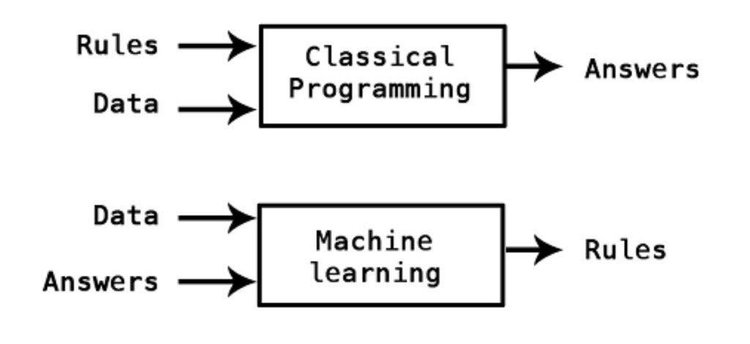
\includegraphics[height=110pt]{../img/ml.jpeg}\\
						From: \href{https://www.manning.com/books/deep-learning-with-python}{Deep Learning with Python}.
					\end{center}

			\end{frame}


			\begin{frame}
				
				\frametitle{Why Debug?}
				
				\begin{itemize}
					
					\item Machine learning models can discriminate, leak private data, get hacked or make silly mistakes.
					
					\item Machine learning pipelines are not magically immune from the bugs and security vulnerabilities that affect all other software.
					
					\item AI incidents can cause harm to organizations, consumers, and the public.
			
				\end{itemize}
			
			\epigraph{“If builders built houses the way programmers built programs, the first woodpecker to come along would destroy civilization.”}{--- \textup{\href{https://en.wikiquote.org/wiki/Gerald_Weinberg}{Gerald Weinberg}}}
				
			\end{frame}


			\begin{frame}

					\frametitle{Why Debug: Inadequate Assessment}

					\begin{columns}
						
						\column{0.5\linewidth}
						\centering
						\begin{itemize}
							\item \scriptsize Constrained, monotonic GBM probability of default (PD) classifier, $g_{\text{mono}}$.
							\item Grid search over hundreds of models. 
							\item Best model selected by validation-based early stopping.
							\item Seemingly well-regularized (row and column sampling, explicit specification of L1 and L2 penalties).
							\item No evidence of over- or under-fitting.
							\item Better validation logloss than benchmark GLM.
							\item Decision threshold selected by maximization of F1 statistic.
							\item BUT traditional assessment can be inadequate ... 
						\end{itemize}\normalsize
						
						\vspace{20pt}
						\column{0.5\linewidth}
							\centering
							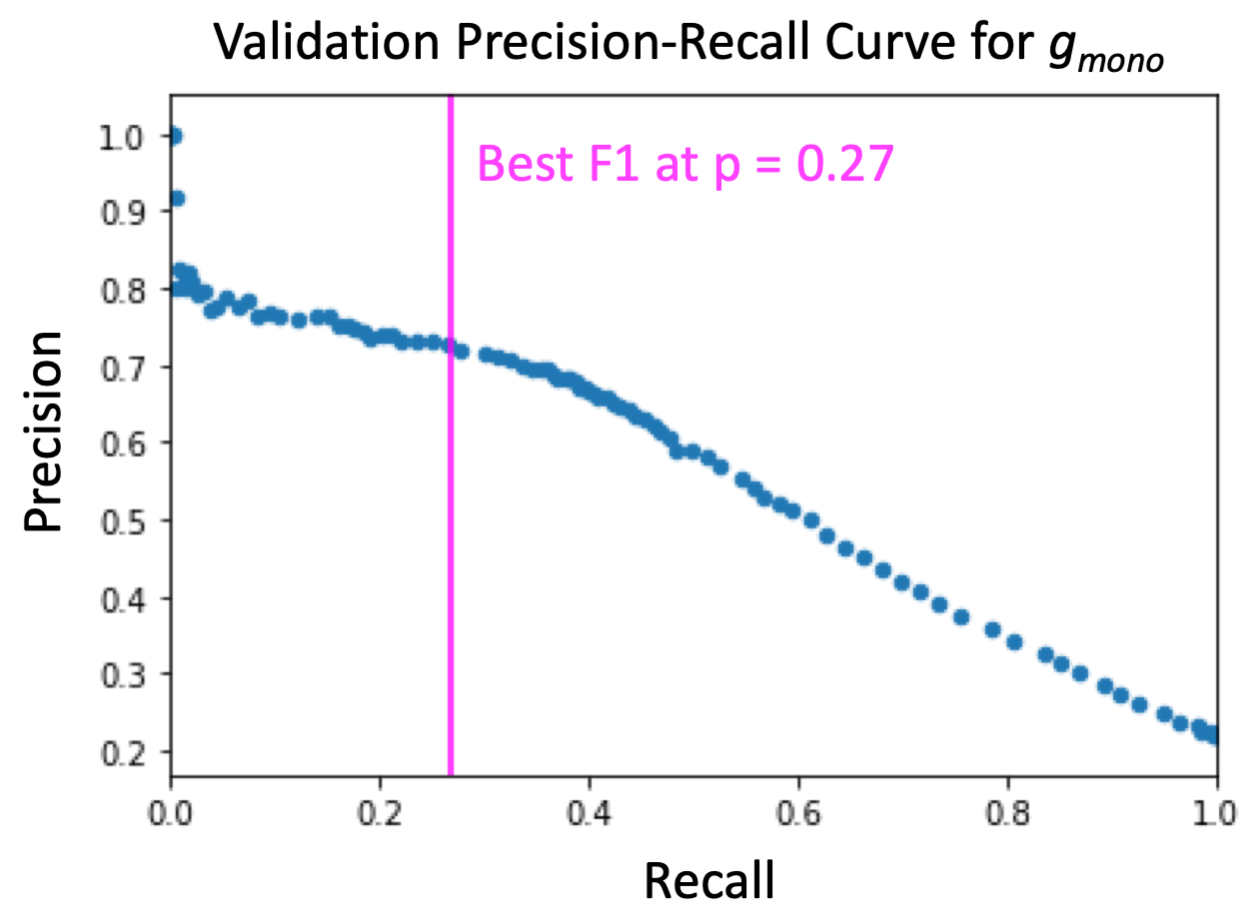
\includegraphics[height=110pt]{../img/pr_auc.png}\\
							\tiny
							\vspace{5pt}
							Validation Confusion Matrix at Threshold:\vspace{-7pt}
							\begin{table}
								\hspace{7pt}
								\begin{tabular}{ | p{1.3cm} | p{1cm} | p{1.3cm} | }
									\hline
								 	& Actual: 1 & Actual: 0 \\ 
									\hline
									Predicted: 1 & 1159	& 827 \\
									\hline
									Predicted: 0 & 1064	& 6004 \\
									\hline
								\end{tabular}	
							\end{table}	
						\normalsize
				
					\end{columns}
							
			\end{frame}

			\begin{frame}
		
				\frametitle{Why Debug: Inaccuracy}
		
					\footnotesize{Machine learning models can be \textbf{inaccurate}.}
					\begin{columns}
				
						\column{0.5\linewidth}
						\centering
						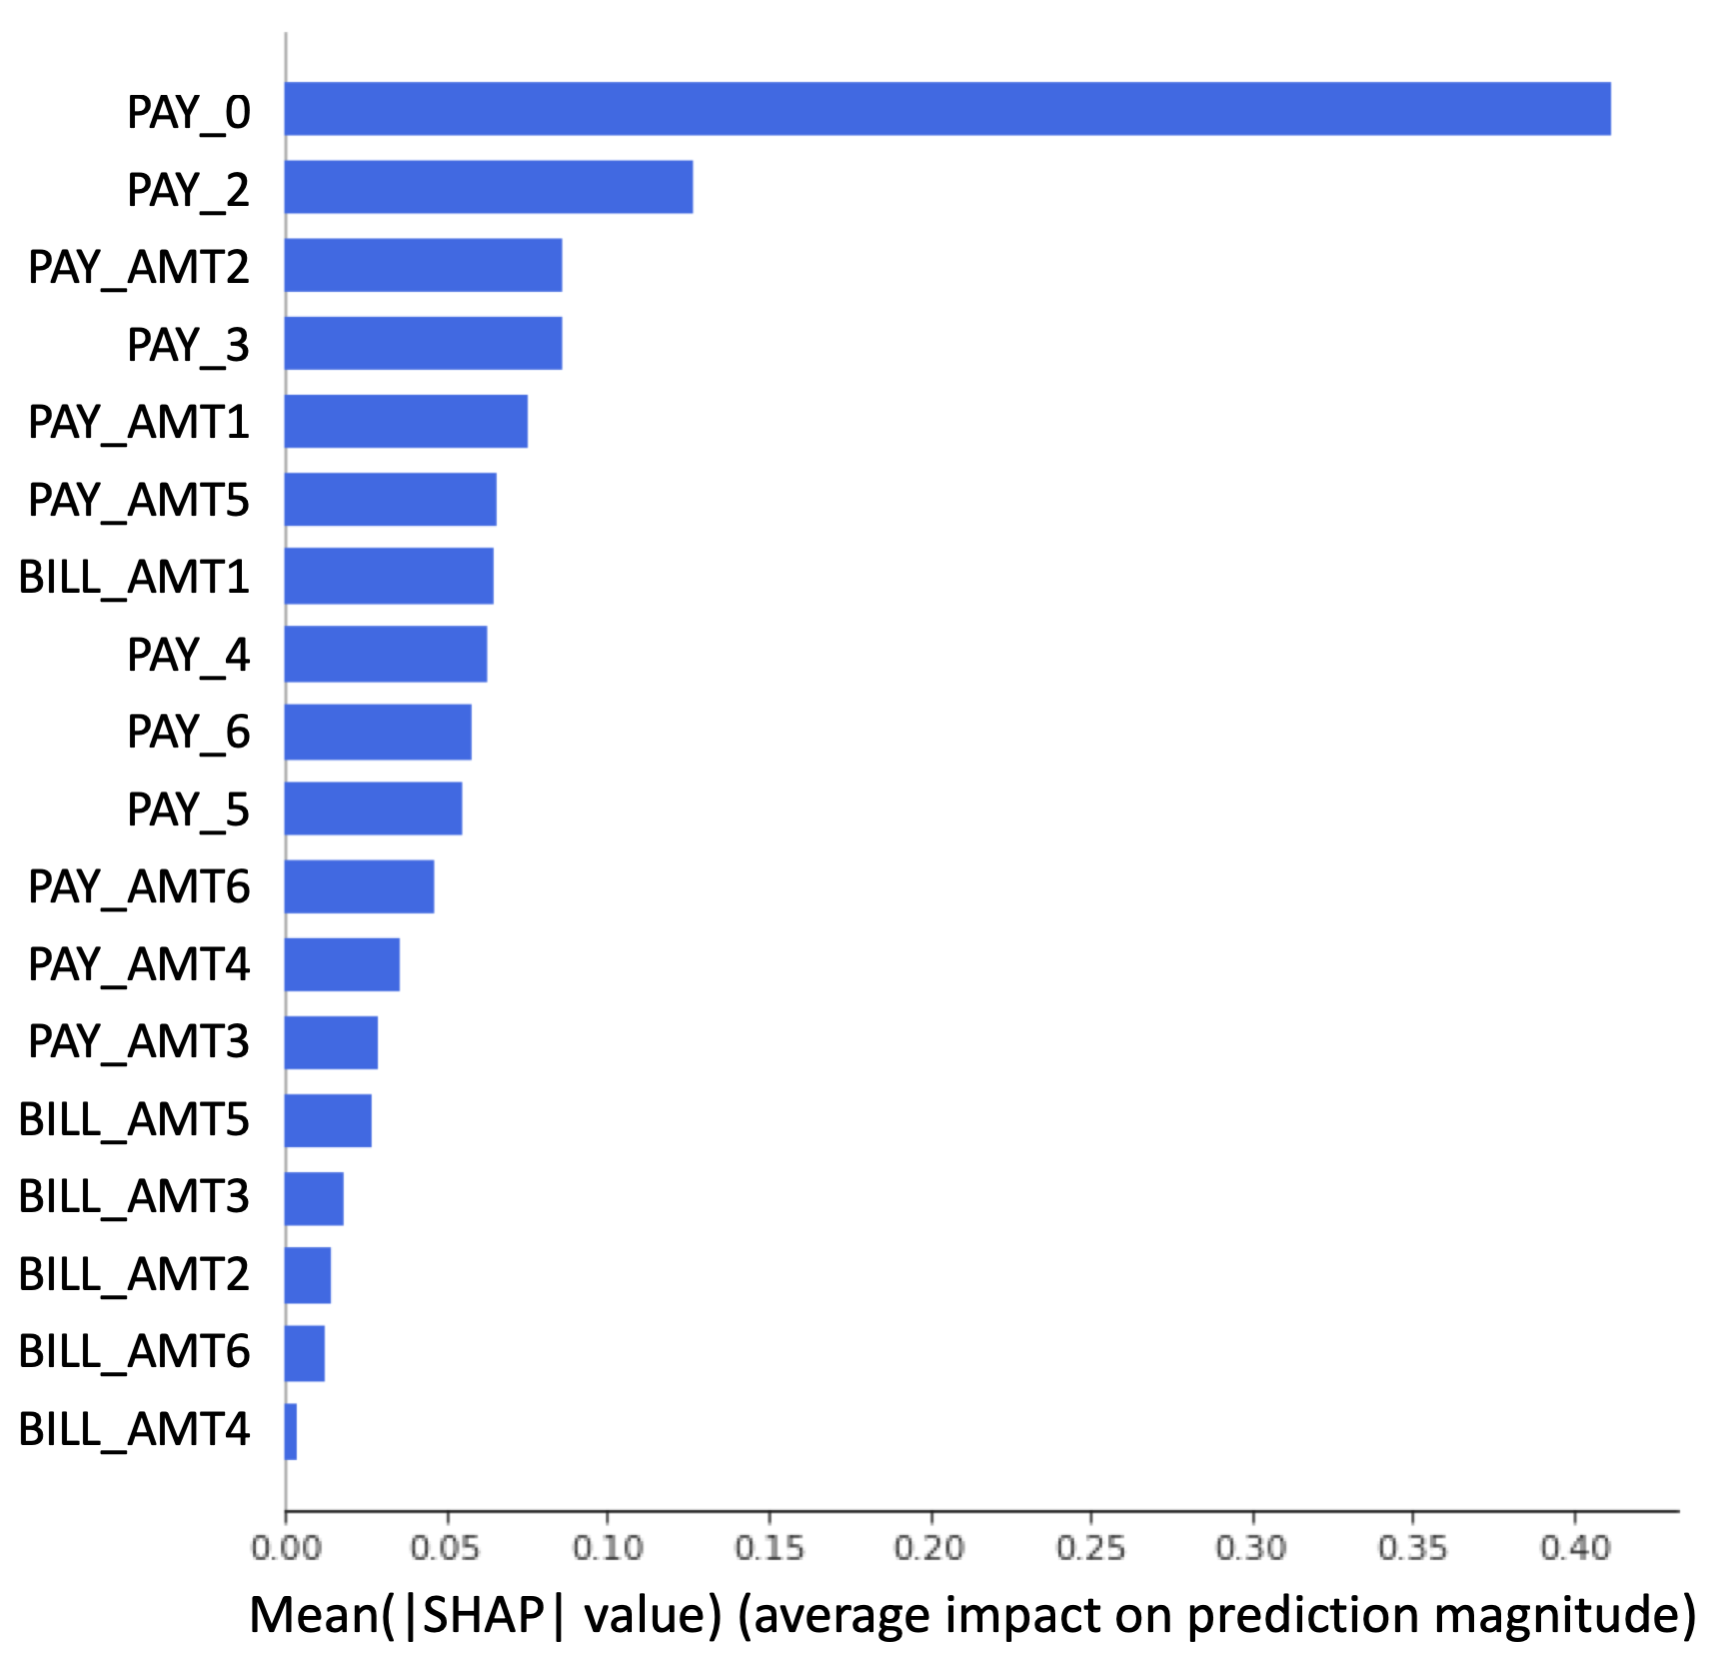
\includegraphics[height=125pt]{../img/global_shap.png}\\
						\vspace{5pt}
						\tiny{$g_{\text{mono}}$ PD classifier over-emphasizes the most important feature, a customer's most recent repayment status, $\text{PAY\_0}$.}

						\vspace{11pt}
						\column{0.5\linewidth}
						\centering
						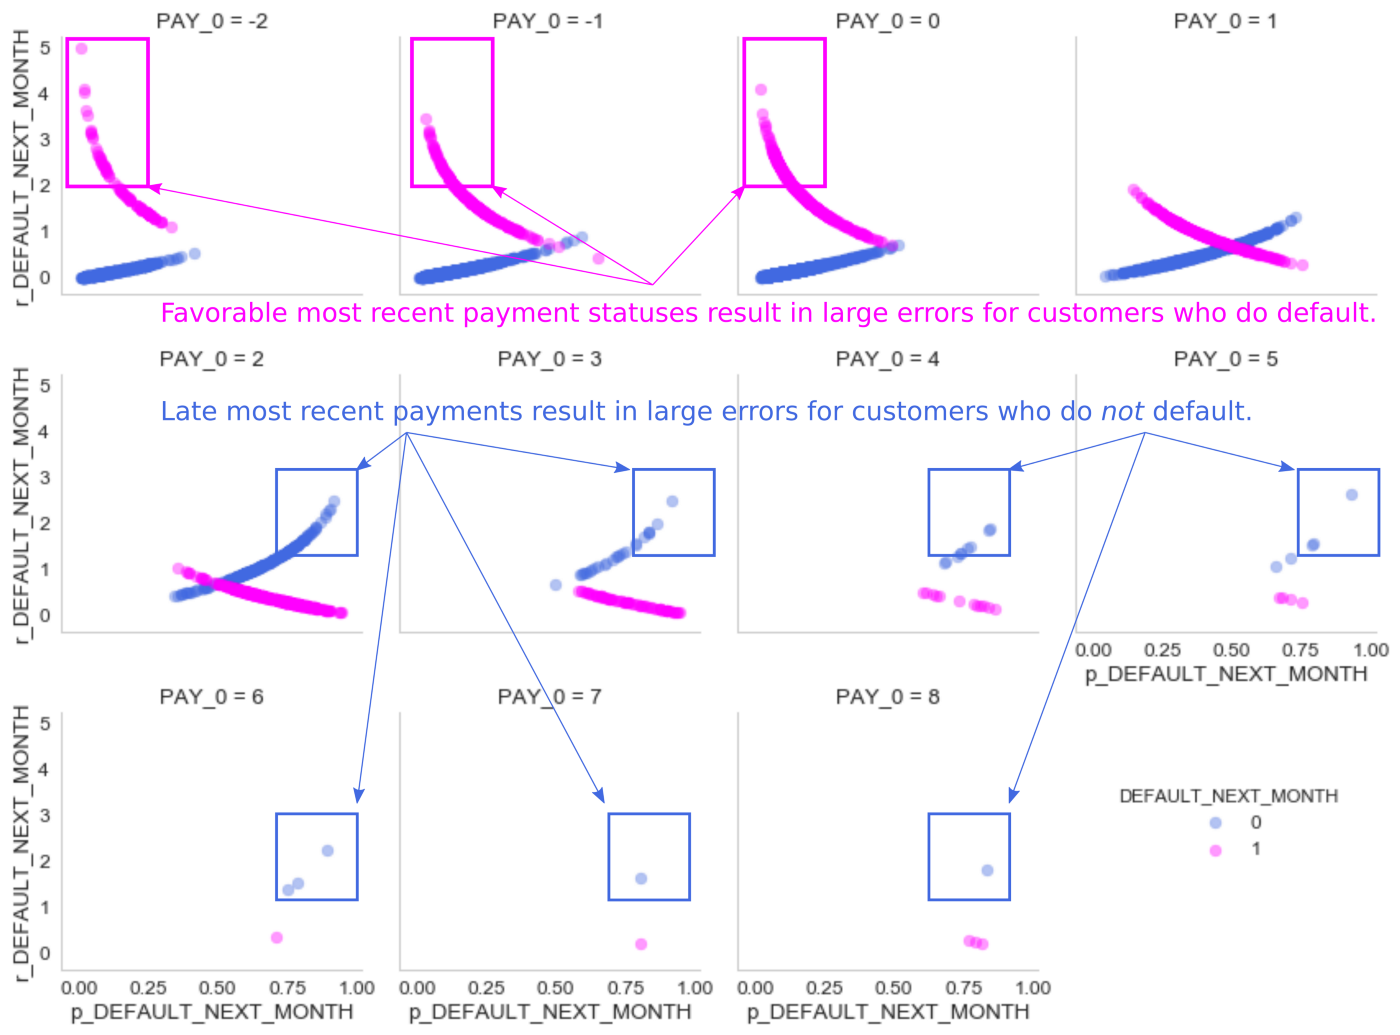
\includegraphics[height=118pt]{../img/lecture_5.png}\\
						\vspace{7pt}
						\tiny{$g_{\text{mono}}$ also struggles to predict default for favorable statuses, $-2  \leq \texttt{PAY\_0}  < 2$, and often cannot predict on-time payment\\when recent payments are late, $\text{PAY\_0} \geq 2$}.
				
					\end{columns}
					\normalsize
			
			\end{frame}
		
			\begin{frame}[label={slide:disp}]
		
				\frametitle{Why Debug: Discrimination}
		
				\footnotesize{Machine learning models can perpetuate \textbf{sociological discrimination} \cite{barocas-hardt-narayanan}.}
				\vspace{10pt}	
				\begin{figure}
					\begin{center}
						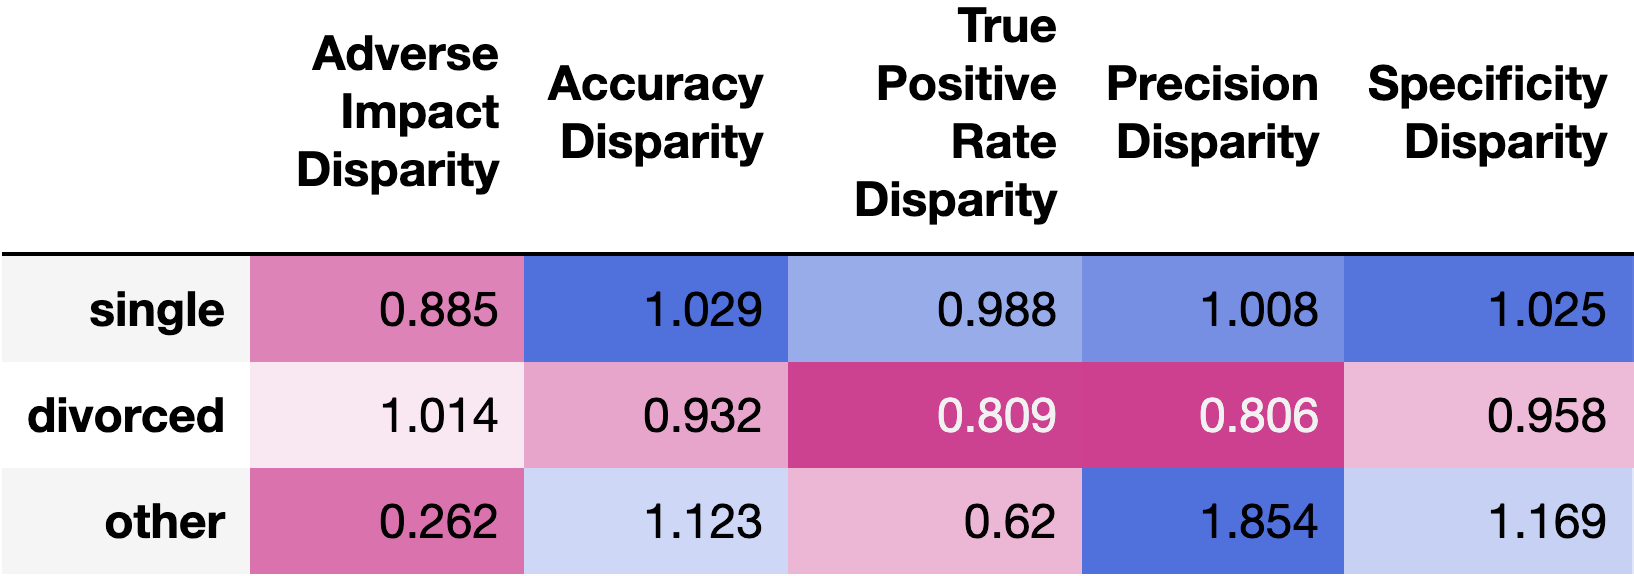
\includegraphics[height=100pt]{../img/di.png}
					\end{center}
				\end{figure}
				\center{\scriptsize{Group disparity metrics are out-of-range for $g_{\text{mono}}$ across different marital statuses.}}
				\normalsize
		
			\end{frame}
		
% Hackers, competitors, or malicious or extorted insiders can manipulate model outcomes, steal models, and steal data!
			\begin{frame}[t]
		
				\frametitle{Why Debug: Security Vulnerabilities}
		
				\footnotesize{Machine learning models have \textbf{security vulnerabilities} \cite{security_of_ml}, \cite{membership_inference}, \cite{model_stealing}}.\footnote{\tiny{See \url{https://github.com/jphall663/secure_ML_ideas} for full size image and more information.}}
				\begin{figure}[]
					\begin{center}
						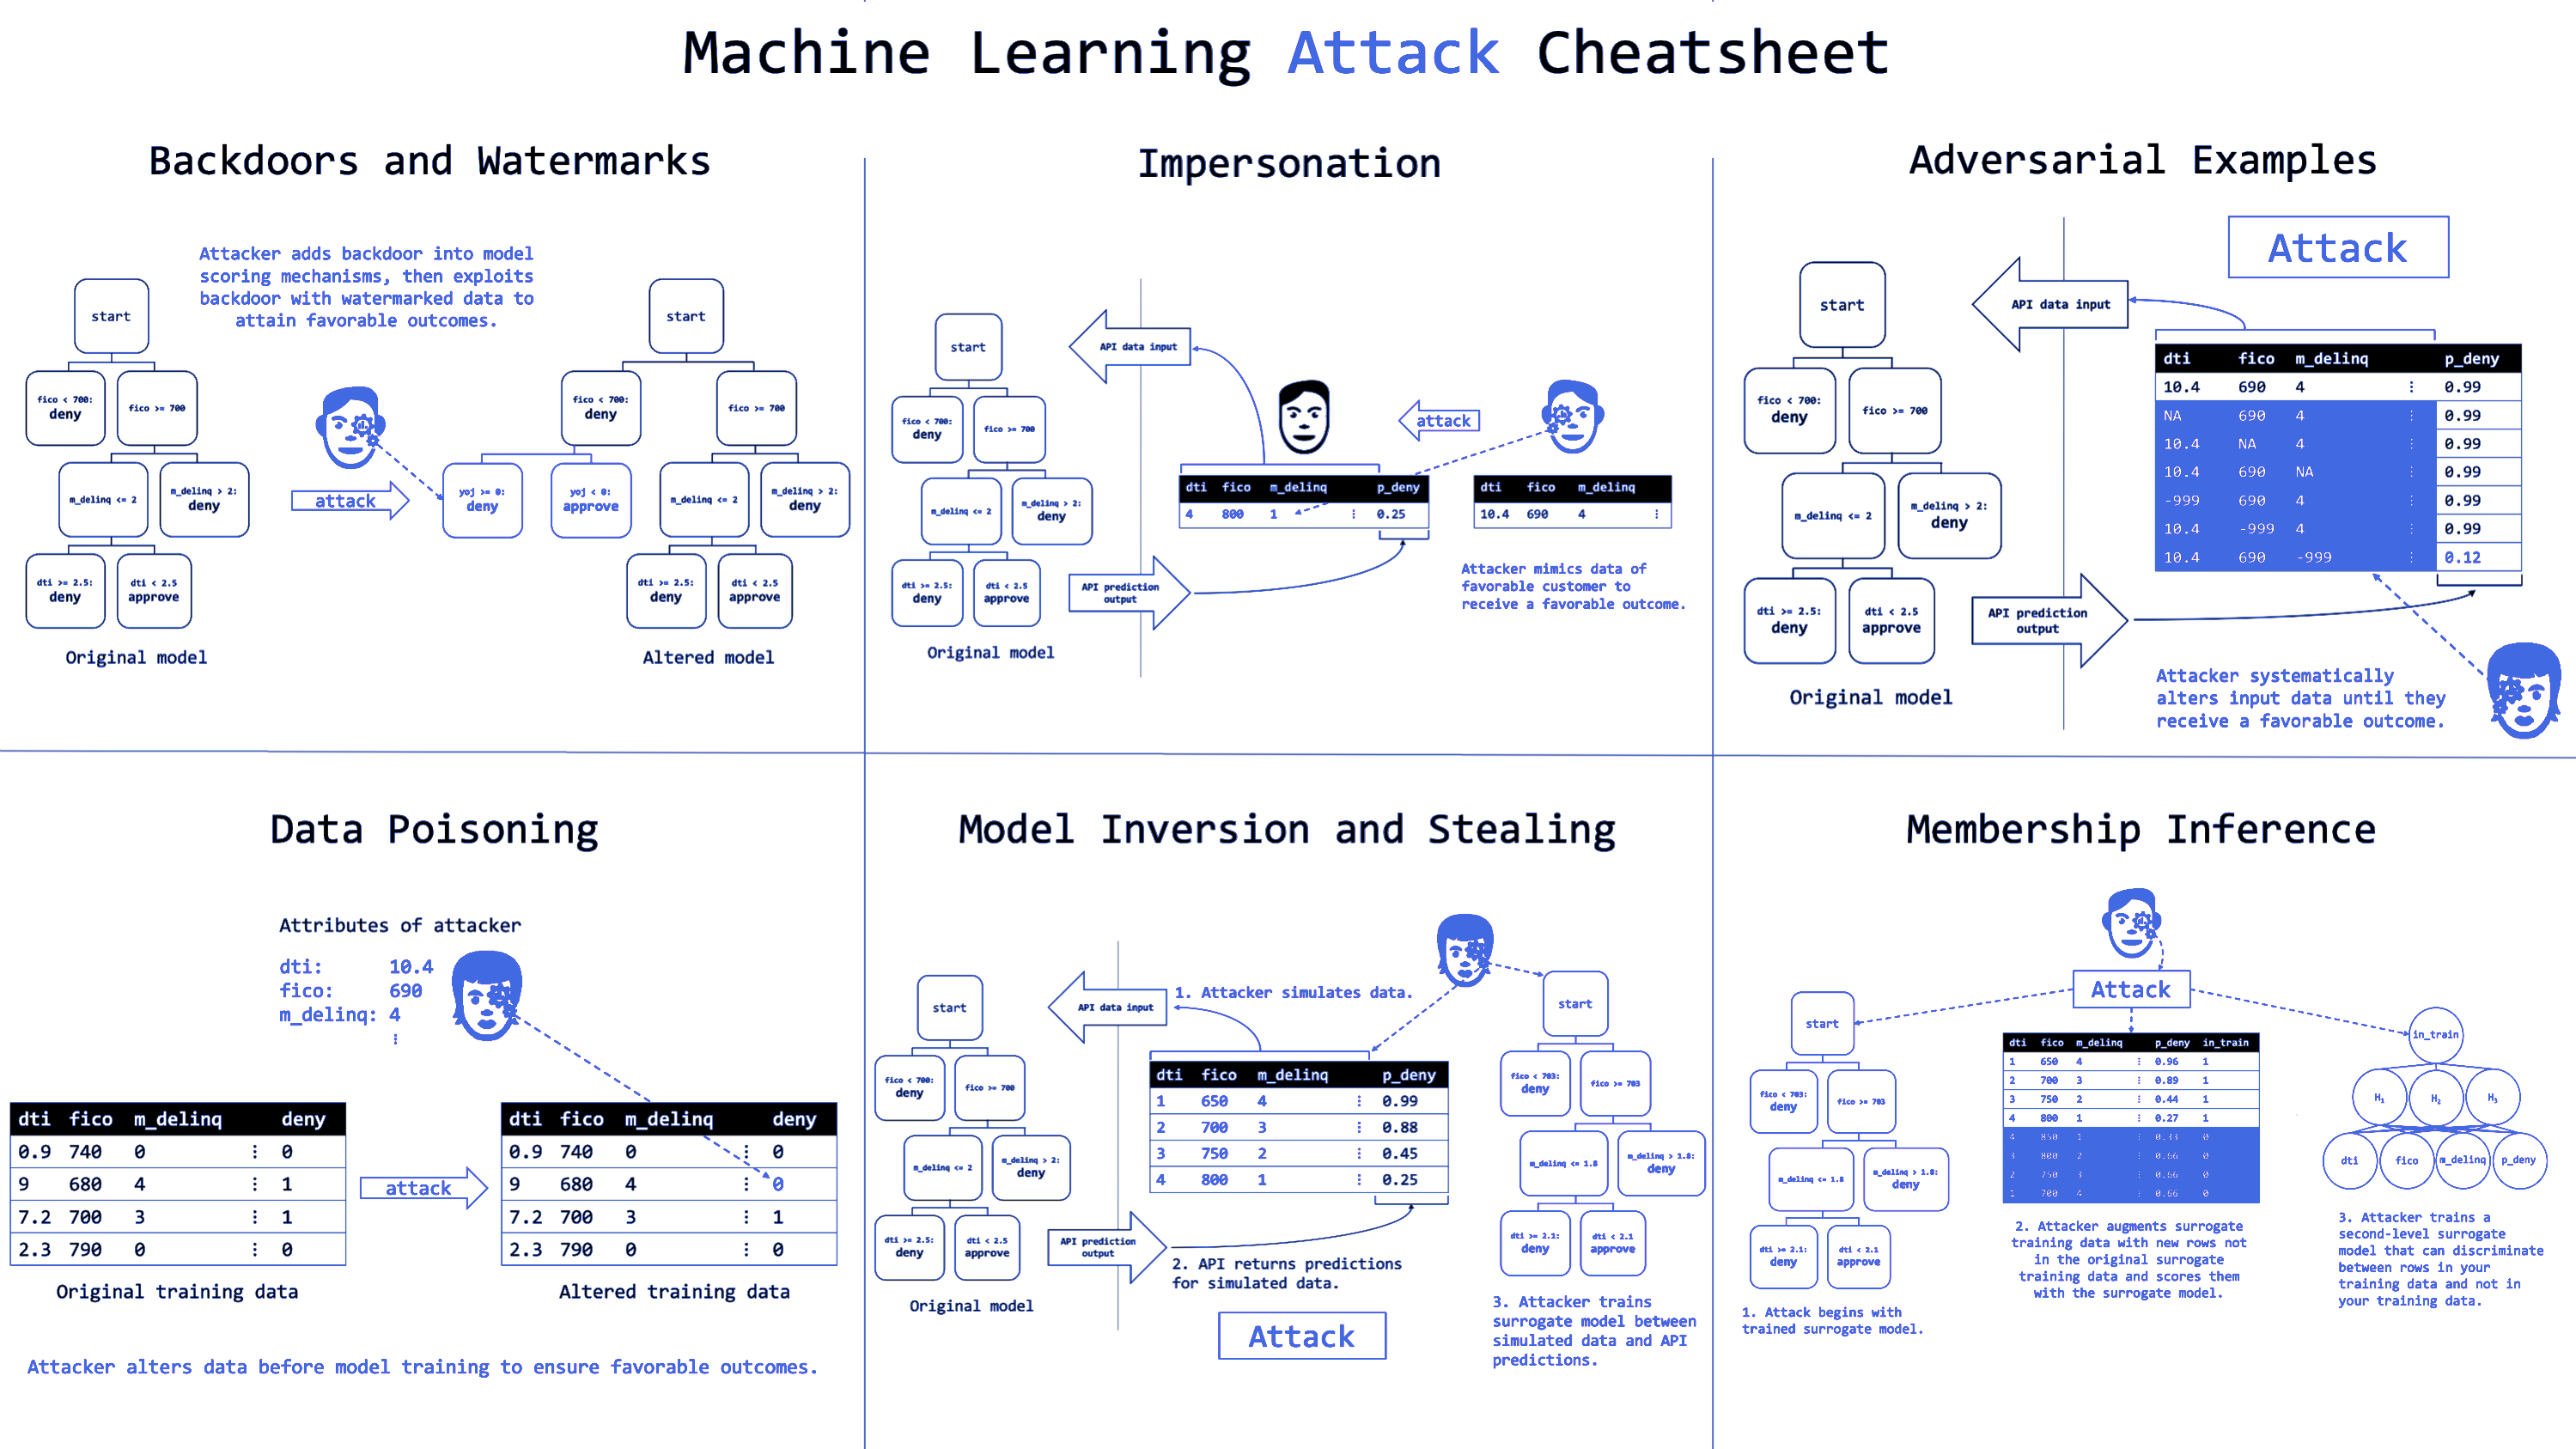
\includegraphics[height=135pt]{../img/cheatsheet_blue.png}
					\end{center}
				\end{figure}	
				\vspace{-17pt}
				\normalsize
		
			\end{frame}

%-------------------------------------------------------------------------------
	\section{Methods of Debugging}
%-------------------------------------------------------------------------------

%-------------------------------------------------------------------------------
		\subsection{Holistic, Low-Risk Approach}
%-------------------------------------------------------------------------------	
	
			\begin{frame}
		
				\frametitle{How to Debug Models}
		
				\footnotesize{As part of a holistic, low-risk approach to machine learning}.\footnote{\tiny{See \url{https://github.com/jphall663/hc_ml} for more information.}}
				\begin{figure}
					\begin{center}
						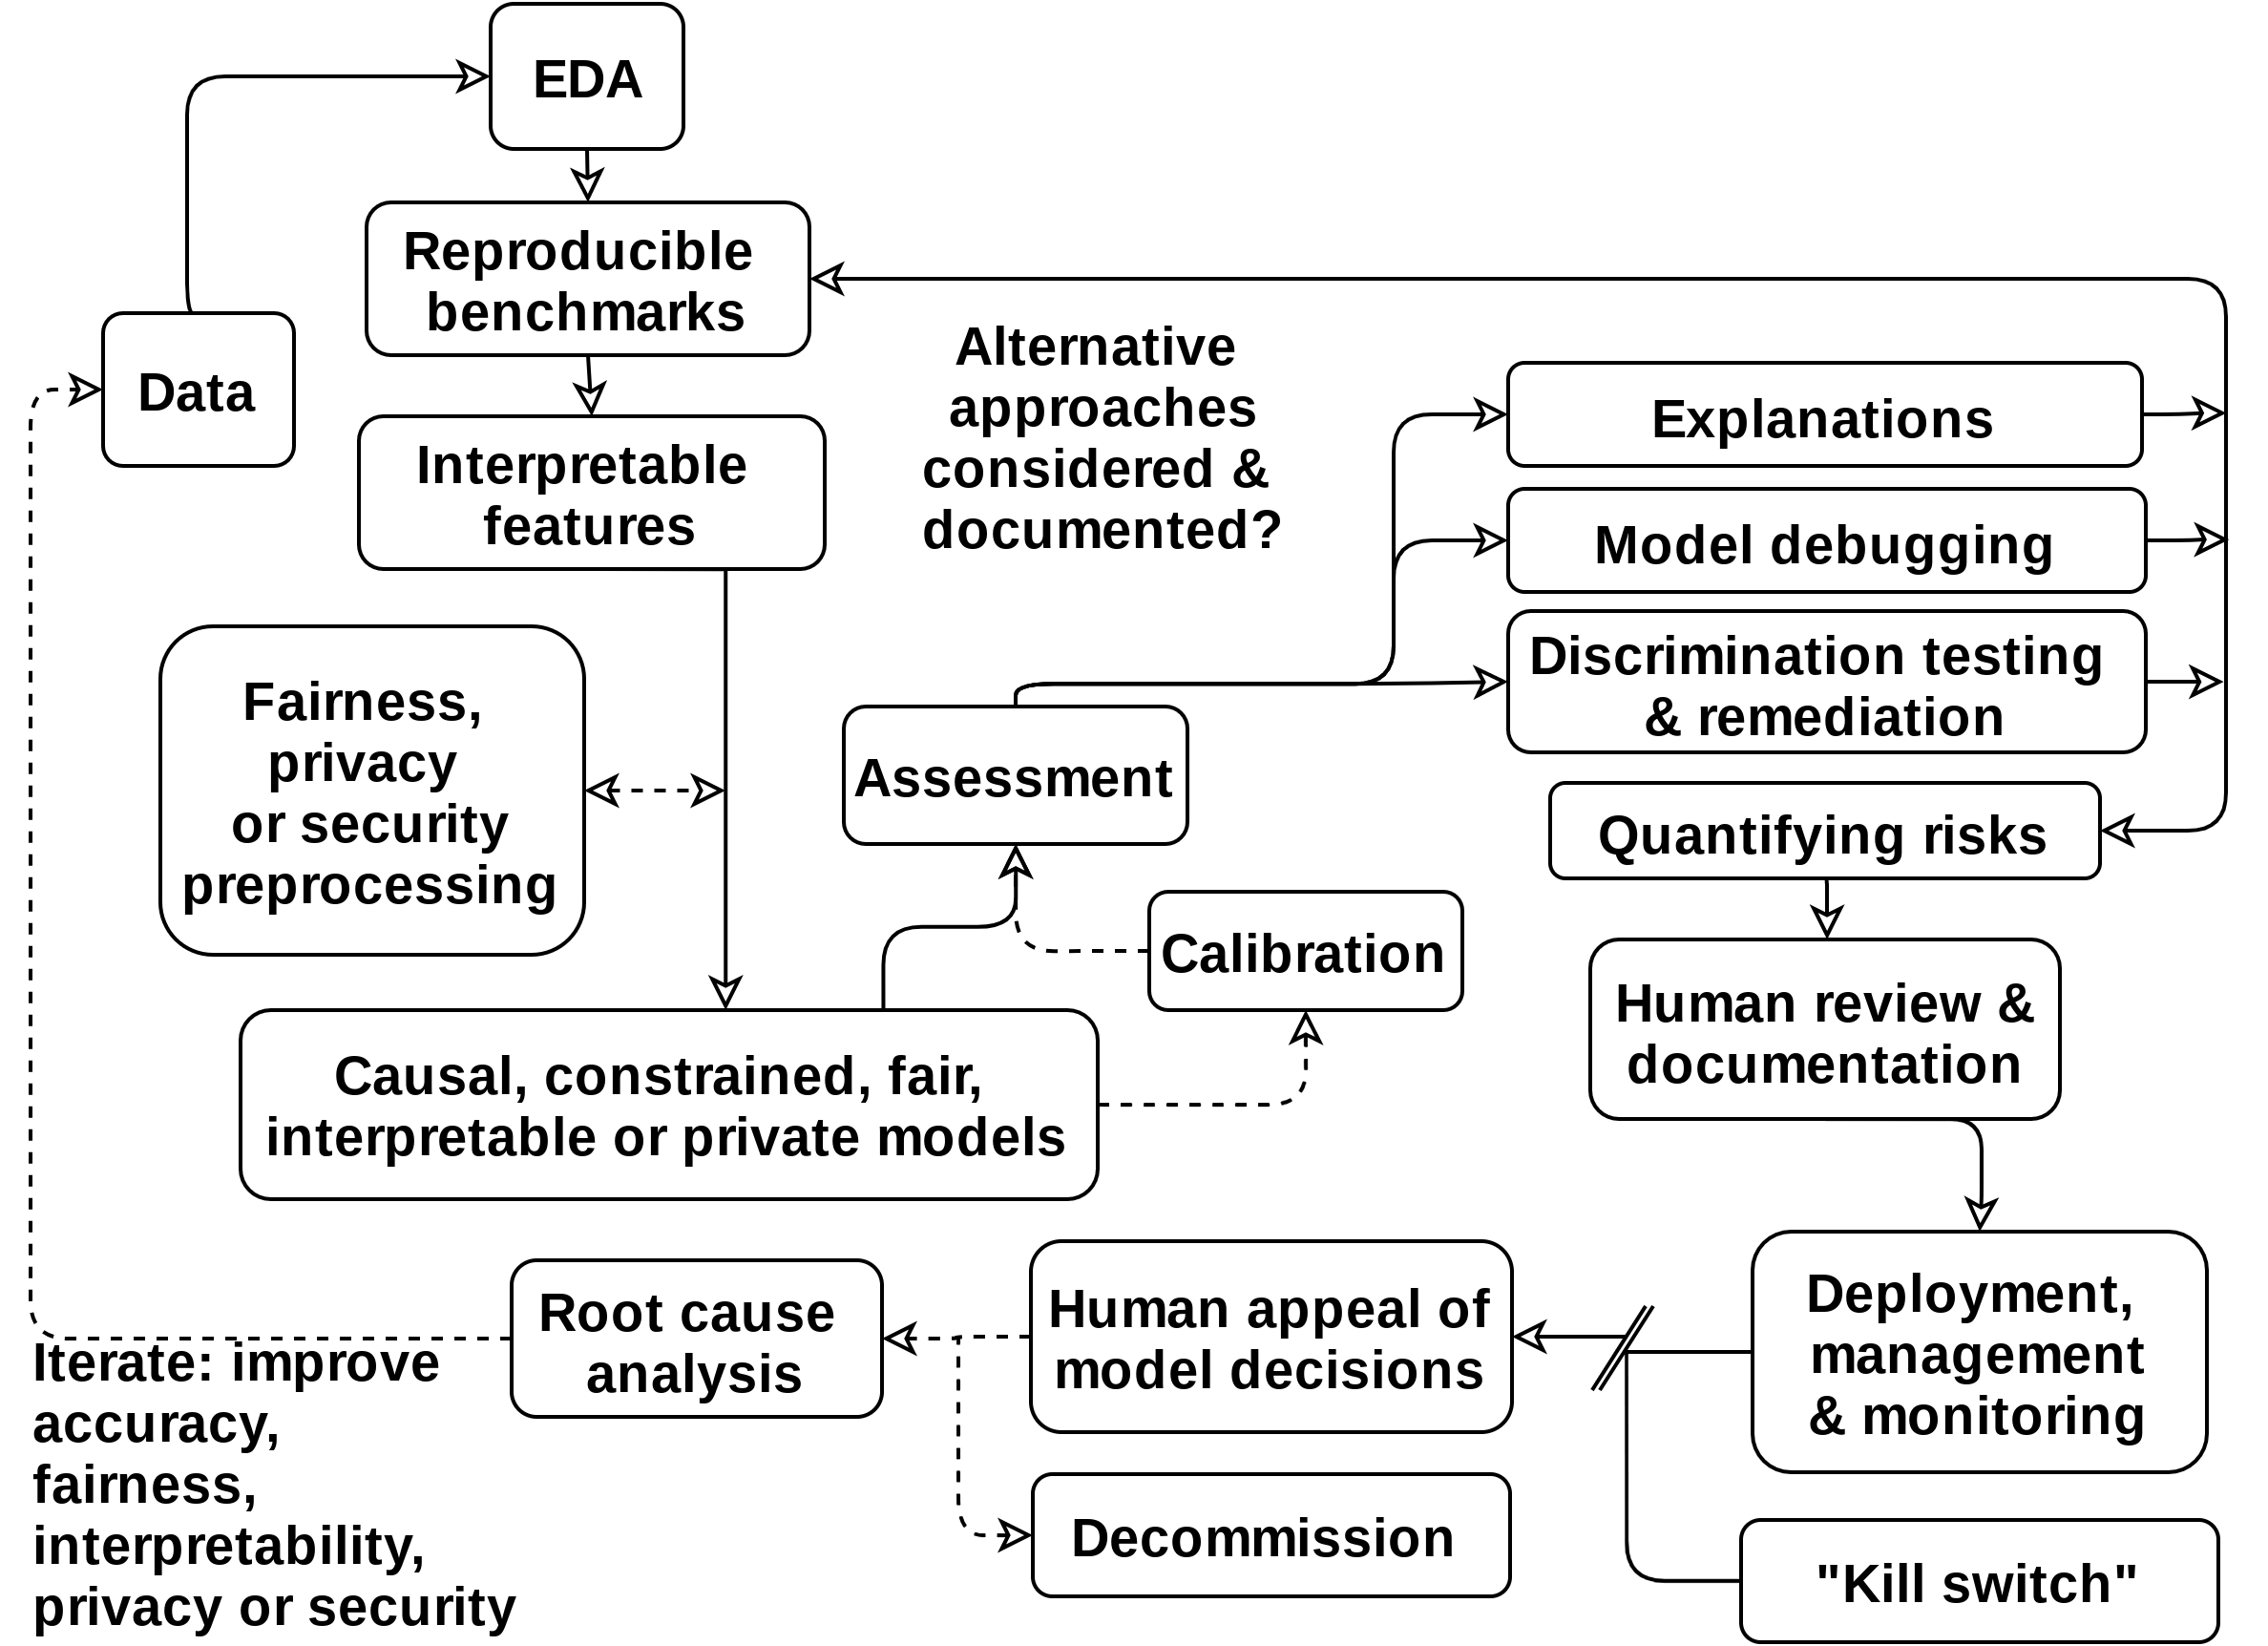
\includegraphics[height=140pt]{../img/rml_diagram_no_hilite.png}
					\end{center}
				\end{figure}	
				\normalsize
		
			\end{frame}

%-------------------------------------------------------------------------------
		\subsection{Sensitivity Analysis}
%-------------------------------------------------------------------------------	

			\begin{frame}[t]
		
				\frametitle{\textbf{Sensitivity Analysis}: Partial Dependence and ICE}
				\vspace{-15pt}
				\begin{figure}
					\begin{center}
						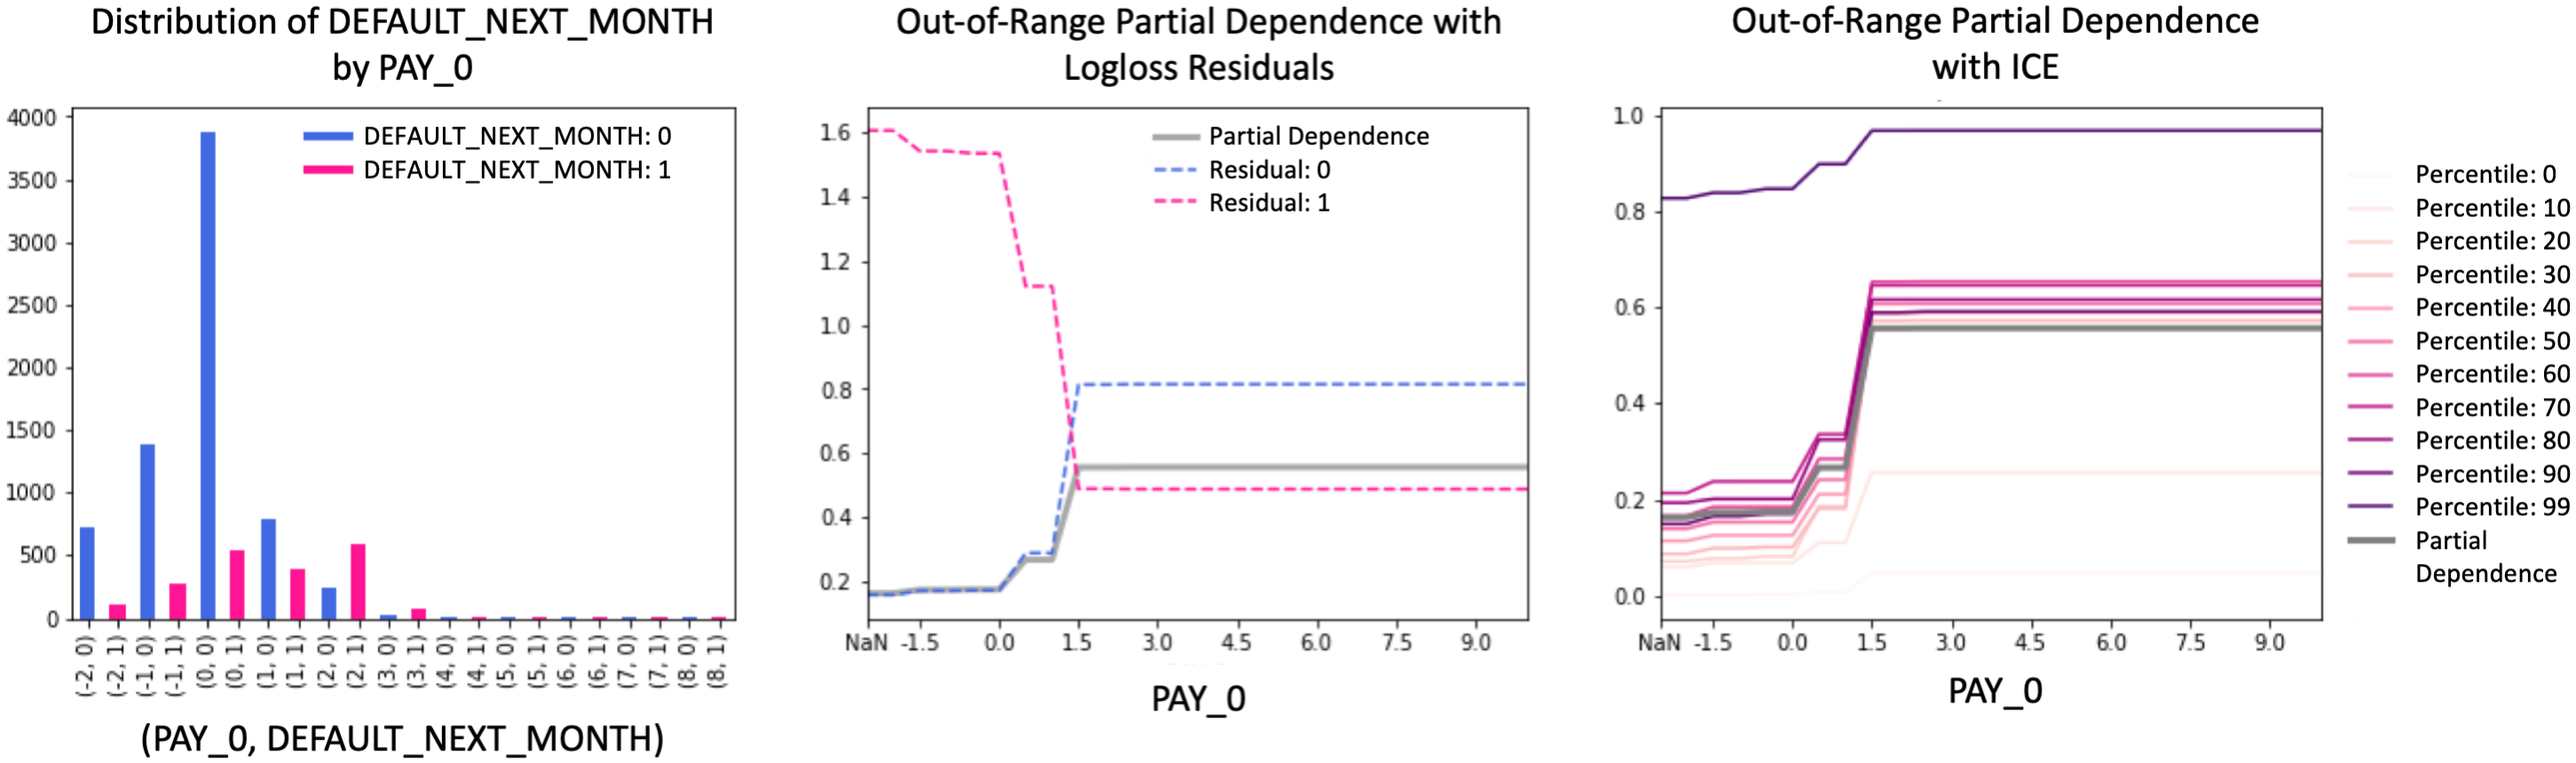
\includegraphics[height=96pt]{../img/pd.png}
					\end{center}
				\end{figure}
				\vspace{-10pt}
				\begin{itemize}	
					\item \scriptsize Training data is very sparse for $\text{PAY\_0} > 2$.\\
					\item Residuals of partial dependence confirm over-emphasis on $\text{PAY\_0}$.
					\item ICE curves indicate that partial dependence is likely trustworthy and empirically confirm monotonicity, but also expose adversarial attack vulnerabilities.
					\item Partial dependence and ICE indicate $g_{\text{mono}}$ likely learned very little for $\text{PAY\_0} \geq 2$.
					\item $\text{PAY\_0} = $ \texttt{missing} gives lowest probability of default.
				\end{itemize}\normalsize
		
			\end{frame}

			\begin{frame}[t, allowframebreaks]
				\vspace{-10pt}
				\frametitle{\textbf{Sensitivity Analysis}: Search for Adversarial Examples}
				\begin{figure}
					\begin{center}
						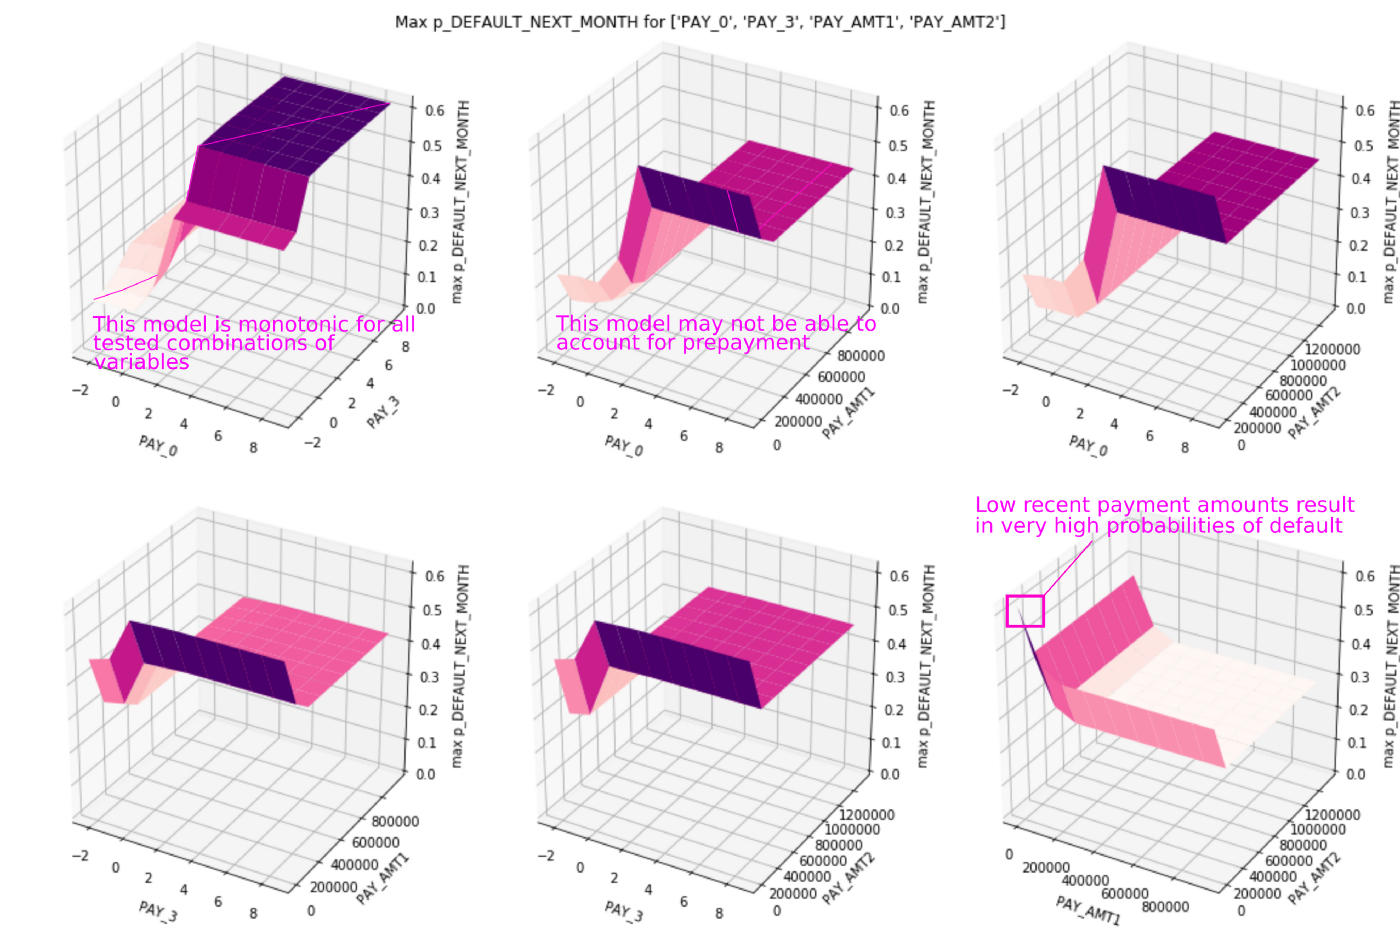
\includegraphics[height=135pt]{../img/sa_max_prob.png}
					\end{center}
				\end{figure}
				\tiny{Adversary search confirms multiple avenues of attack and exposes a potential flaw in $g_{\text{mono}}$ scoring logic: default is predicted for customer's who make payments above their credit limit. (Try the \href{https://github.com/tensorflow/cleverhans}{cleverhans} package for finding adversarial examples.)}
					
				\framebreak
				\vspace{-5pt}
				\begin{figure}
					\begin{center}
						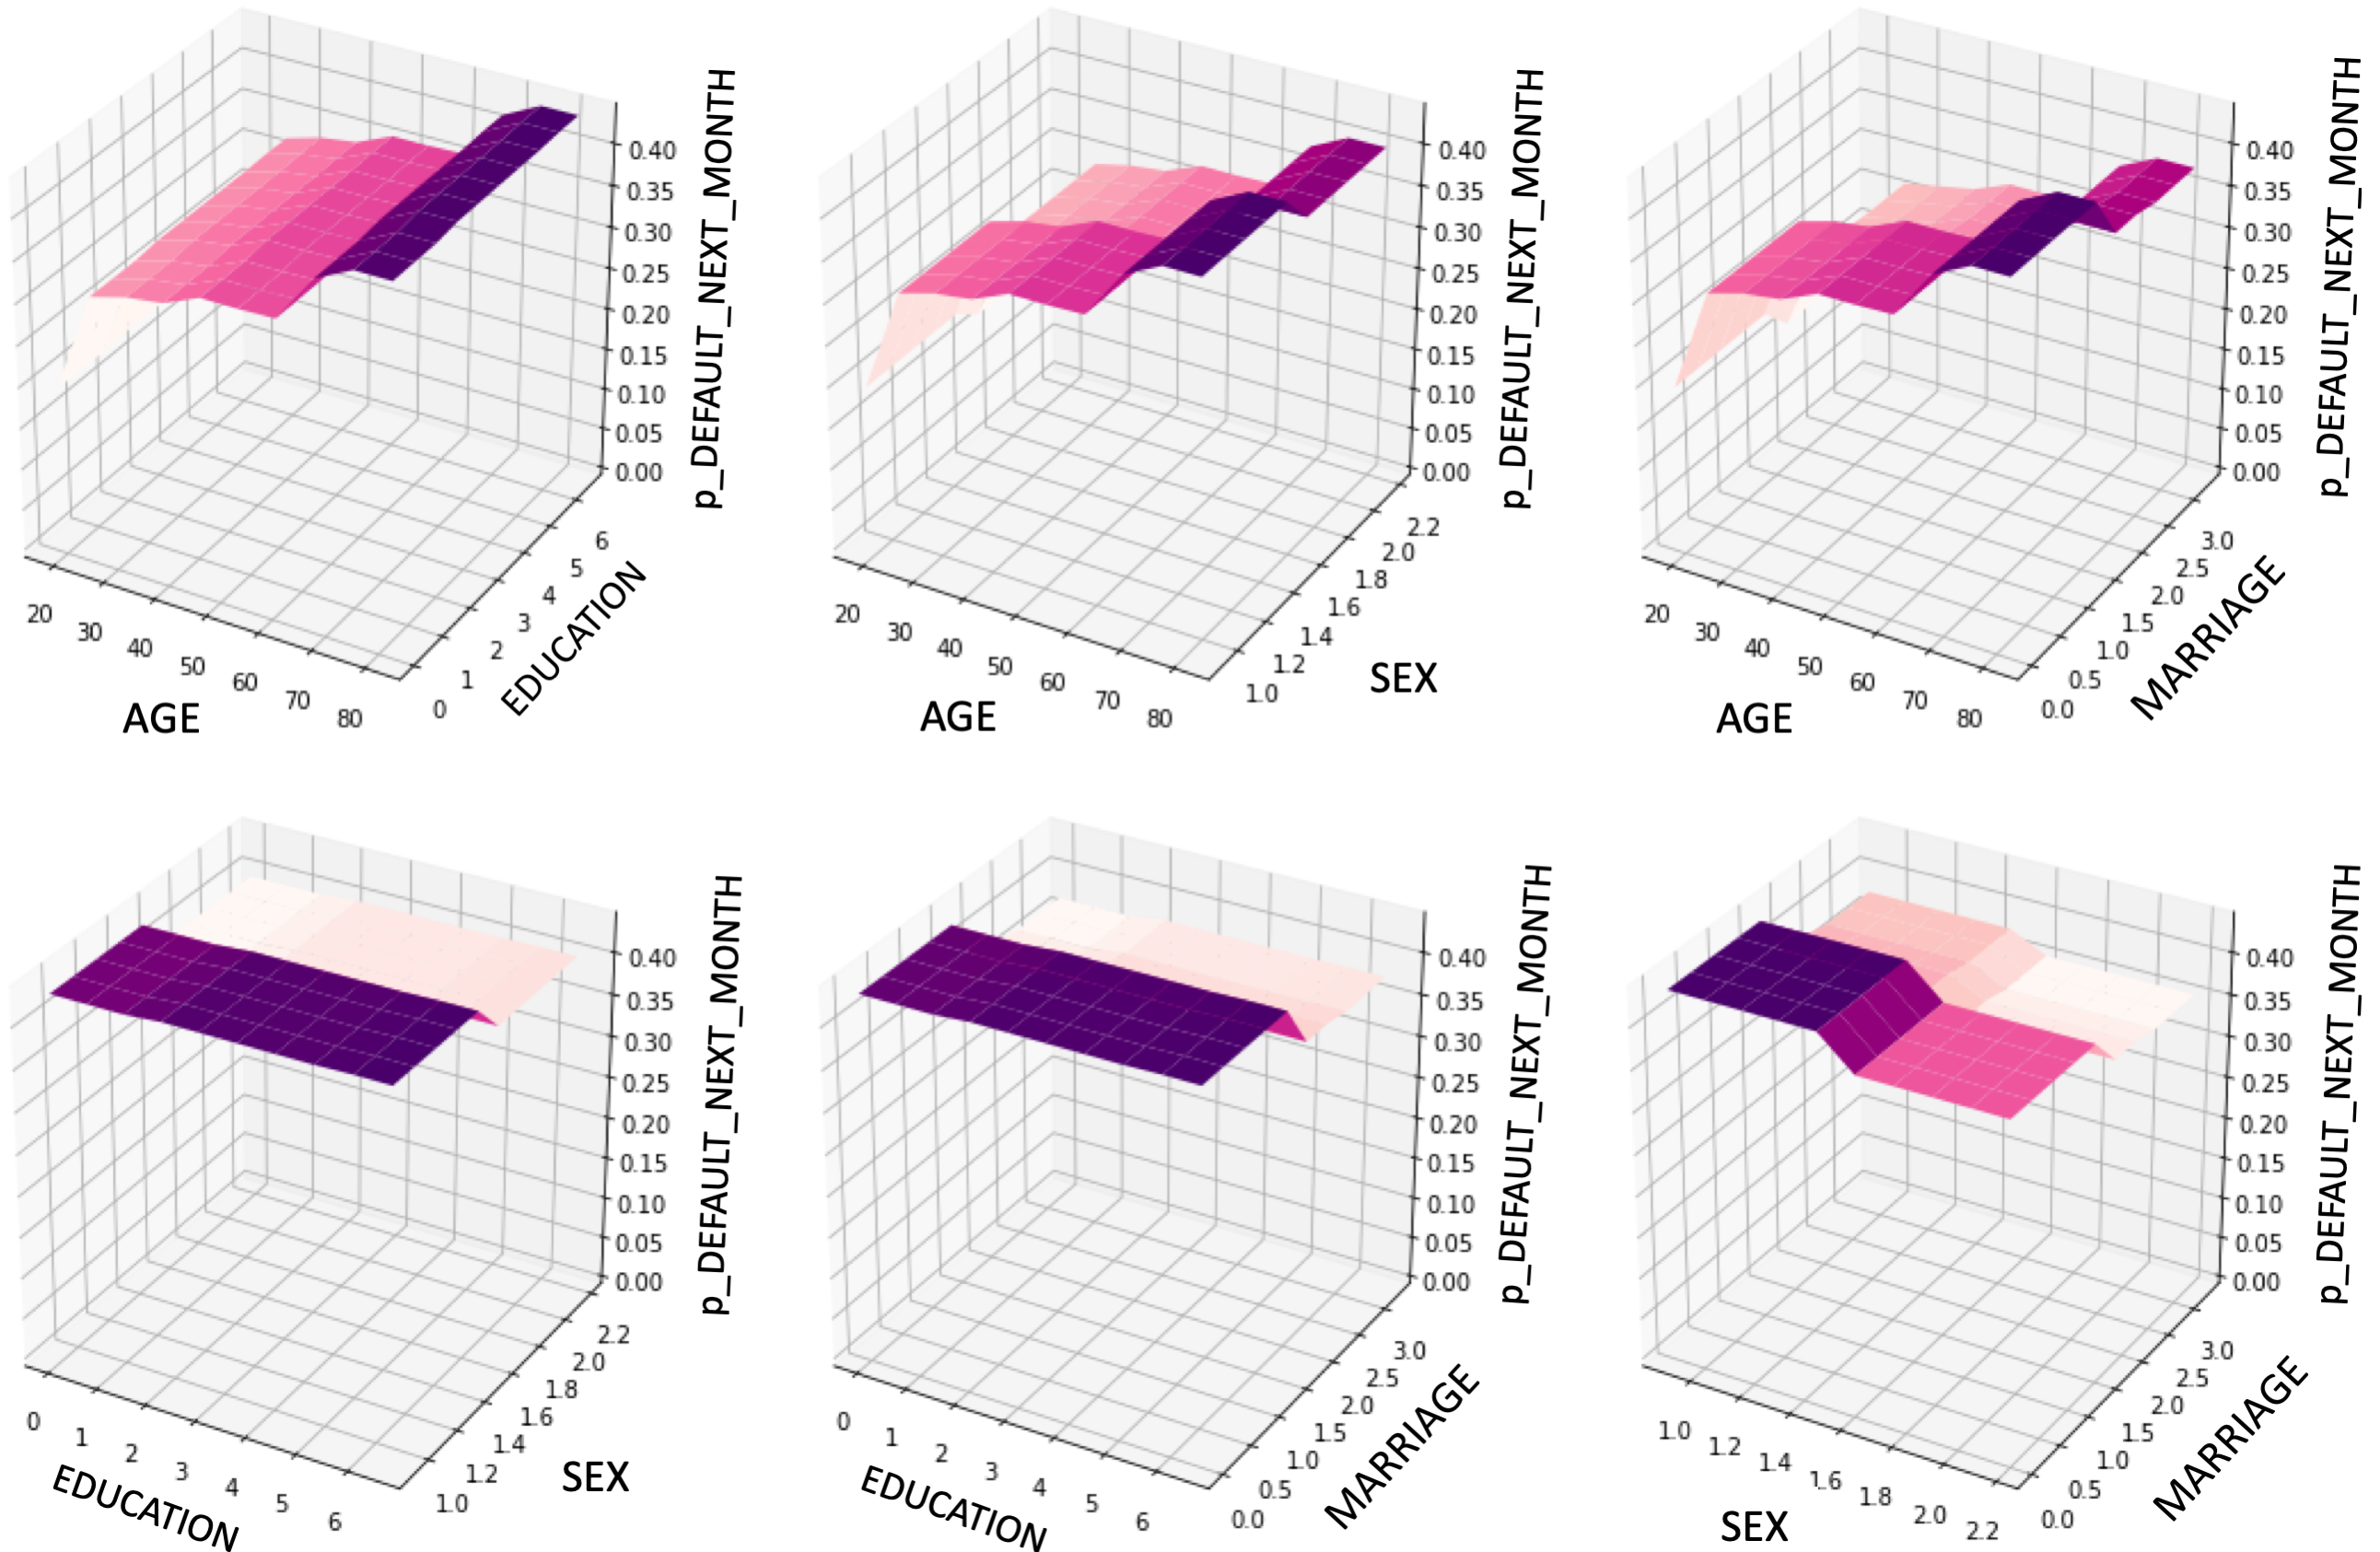
\includegraphics[height=135pt]{../img/sa_max_prob_demo.png}
					\end{center}
				\end{figure}
				\vspace{-5pt}
				\tiny{$g_{\text{mono}}$ appears to prefer younger, unmarried customers, which should be investigated further with disparate impact analysis - see slide \ref{slide:disp} - and could expose the lender to impersonation attacks. (Try the \href{https://github.com/IBM/AIF360}{AIF360}, \href{https://github.com/dssg/aequitas}{aequitas}, or \href{https://github.com/LASER-UMASS/Themis}{themis} packages for disparate impact audits.)}
		
			\end{frame}			
			
			\begin{frame}[t]
		
				%When you don't know what to test
		
				\frametitle{\textbf{Sensitivity Analysis}: Random Attacks}
				\vspace{-15pt}
				\begin{figure}
					\begin{center}
						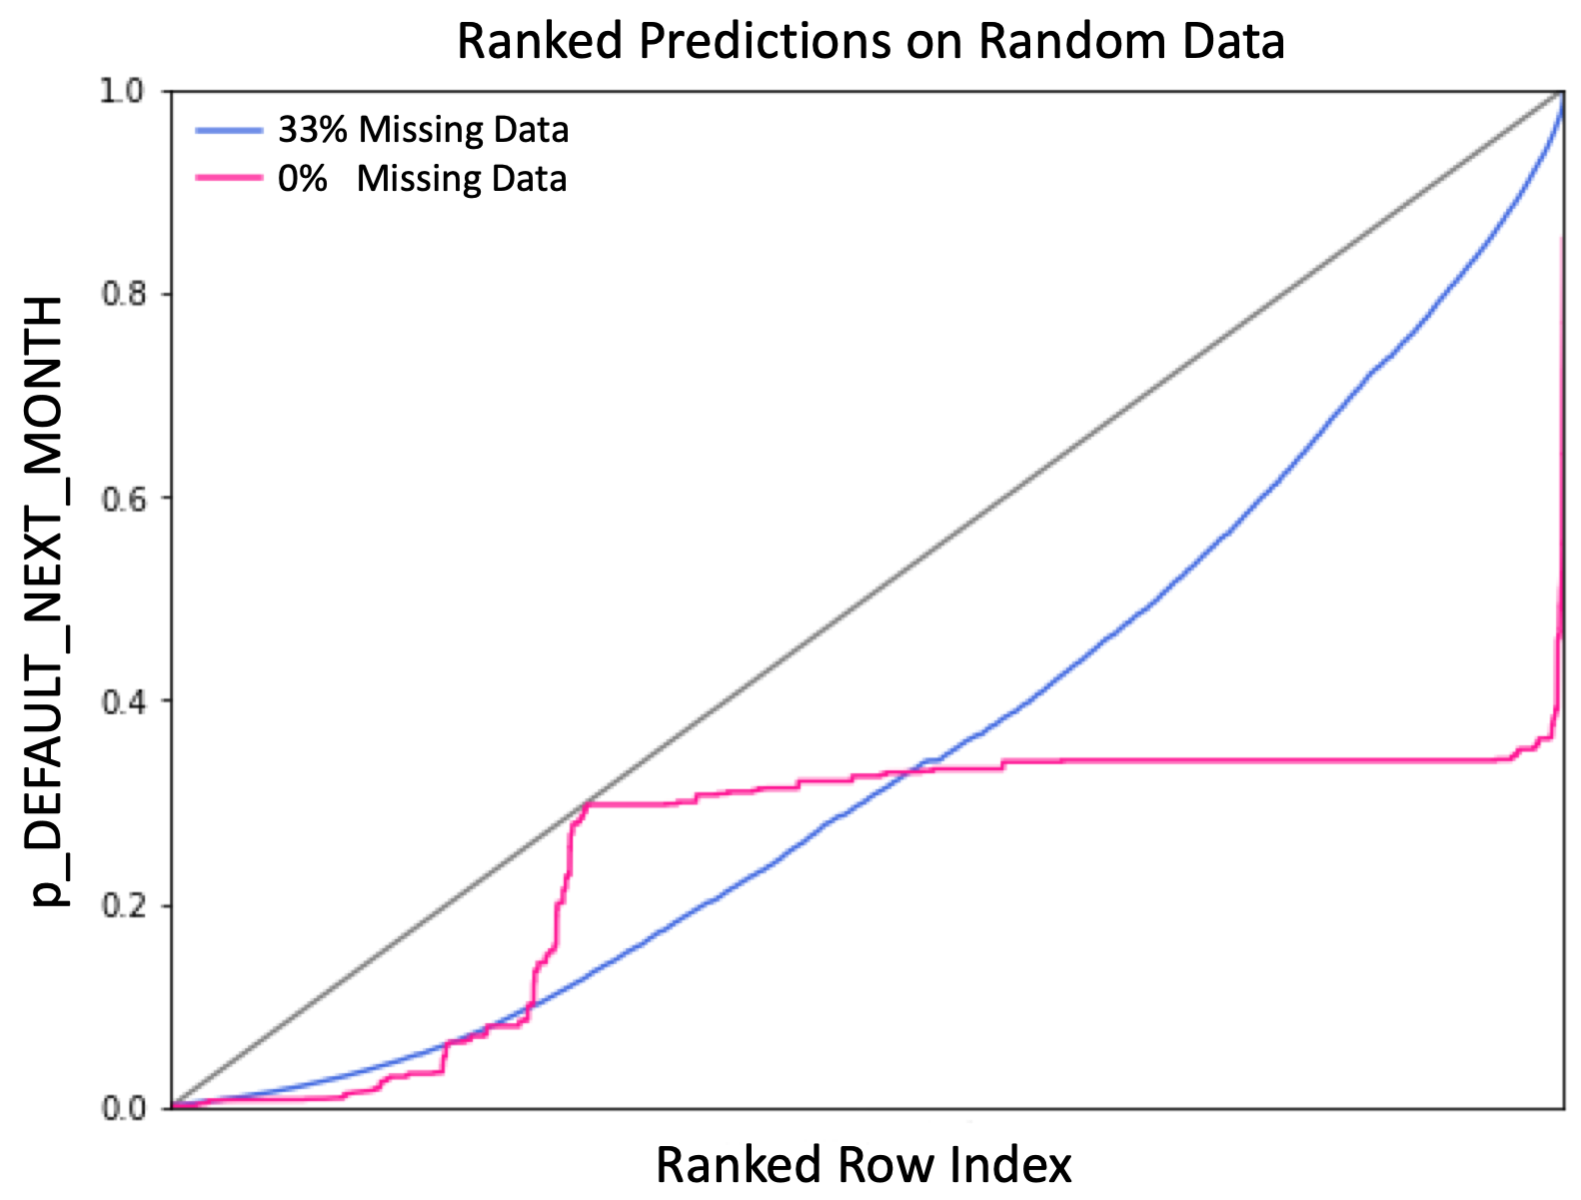
\includegraphics[height=130pt]{../img/ra.png}
					\end{center}
				\end{figure}	
				\vspace{-10pt}
				\begin{itemize}\scriptsize
					\item In general, random attacks are a viable method to identify software bugs in machine learning pipelines. \textbf{(Start here if you don't know where to start.)}
					\item Random data can apparently elicit all probabilities $\in [0, 1]$ from $g_{\text{mono}}$.
					\item Around the decision threshold, lower probabilities can be attained simply by injecting missing values, yet another vulnerability to adversarial attack.
				\end{itemize}
				\normalsize
		
			\end{frame}
			
%-------------------------------------------------------------------------------
		\subsection{Residual Analysis}
%-------------------------------------------------------------------------------	

			\begin{frame}[t]
		
				\frametitle{\textbf{Residual Analysis}: Disparate Accuracy and Errors}
		
		                 \vspace{-10pt}
				\begin{figure}
					\begin{center}
						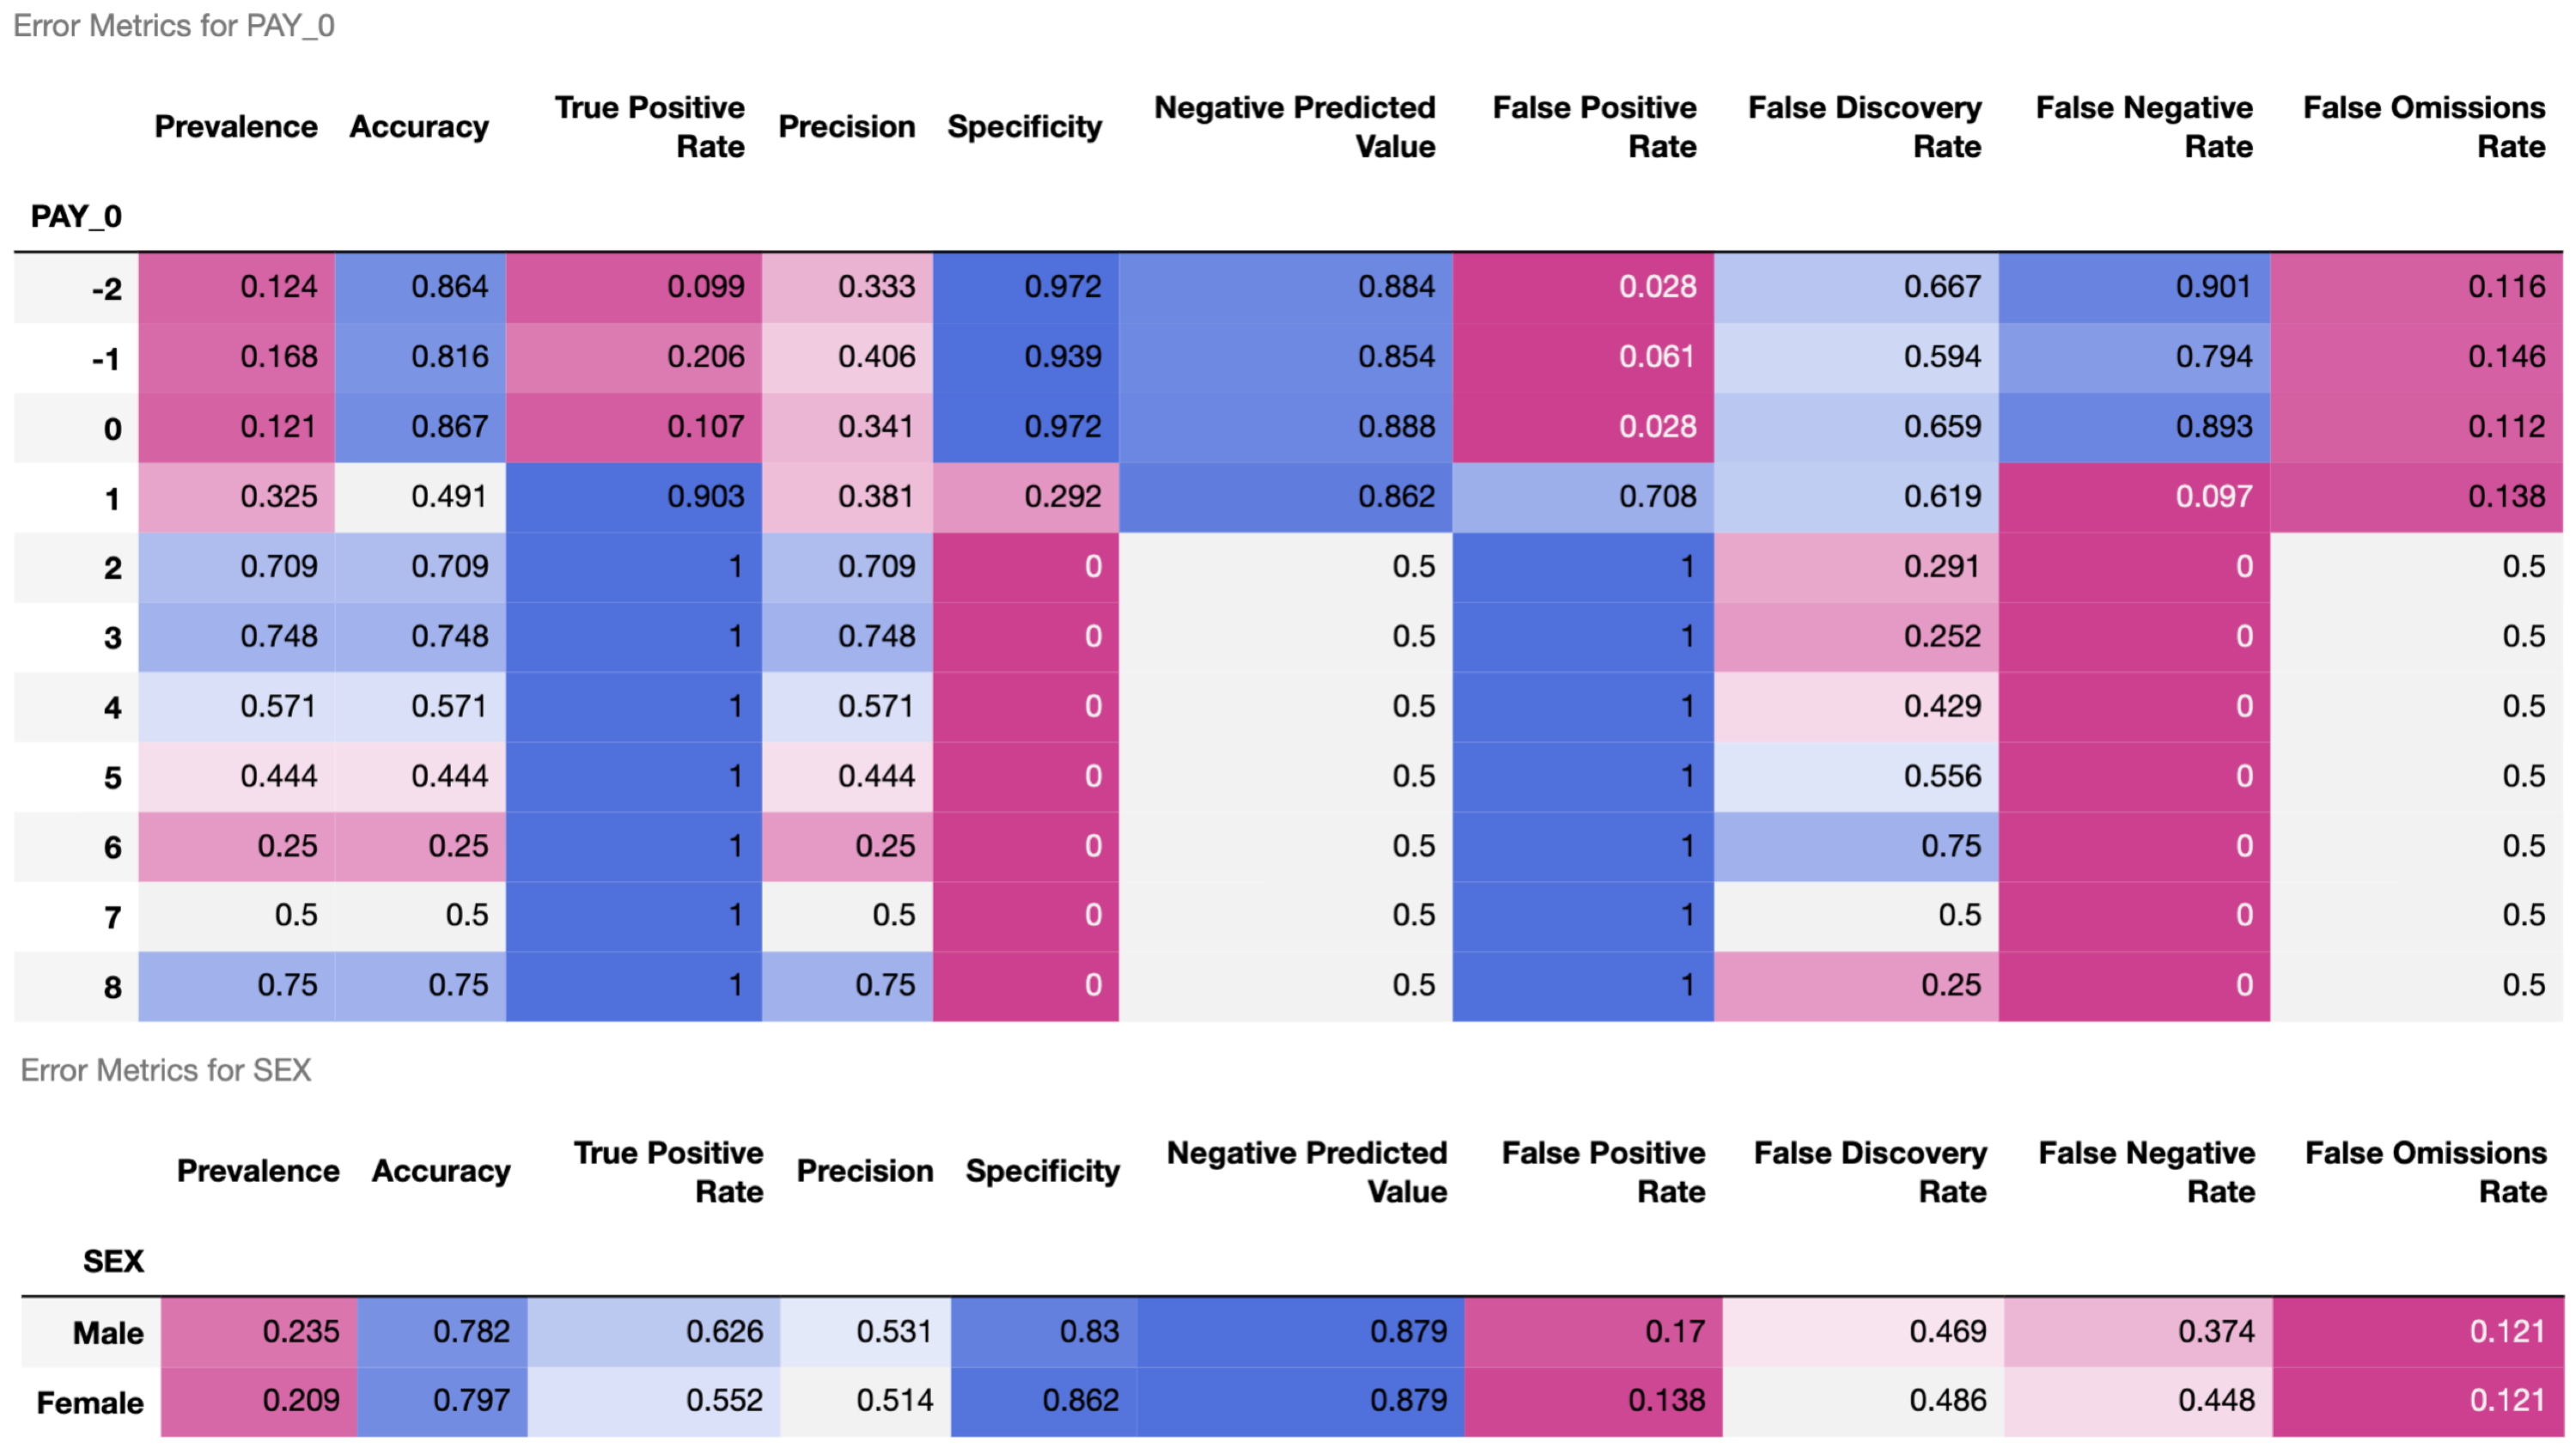
\includegraphics[height=140pt]{../img/de.png}
					\end{center}
				\end{figure}
				\vspace{-15pt}
				\tiny For $\text{PAY\_0}$:
				\begin{itemize}
					\item Notable change in accuracy and error characteristics for $\text{PAY\_0} \geq 2$. 
					\item 100\% false omission rate for $\text{PAY\_0} \geq 2$. (Every prediction of non-default is incorrect!)
				\end{itemize}
				For $\text{SEX}$, accuracy and error characteristics vary little across individuals represented in the training data. Non-discrimination should be confirmed by disparate impact analysis.
		
			\end{frame}

			\begin{frame}[t]
		
				\frametitle{\textbf{Residual Analysis}: Mean Local Feature Contributions}
				\vspace{-15pt}
				\begin{figure}
					\begin{center}
						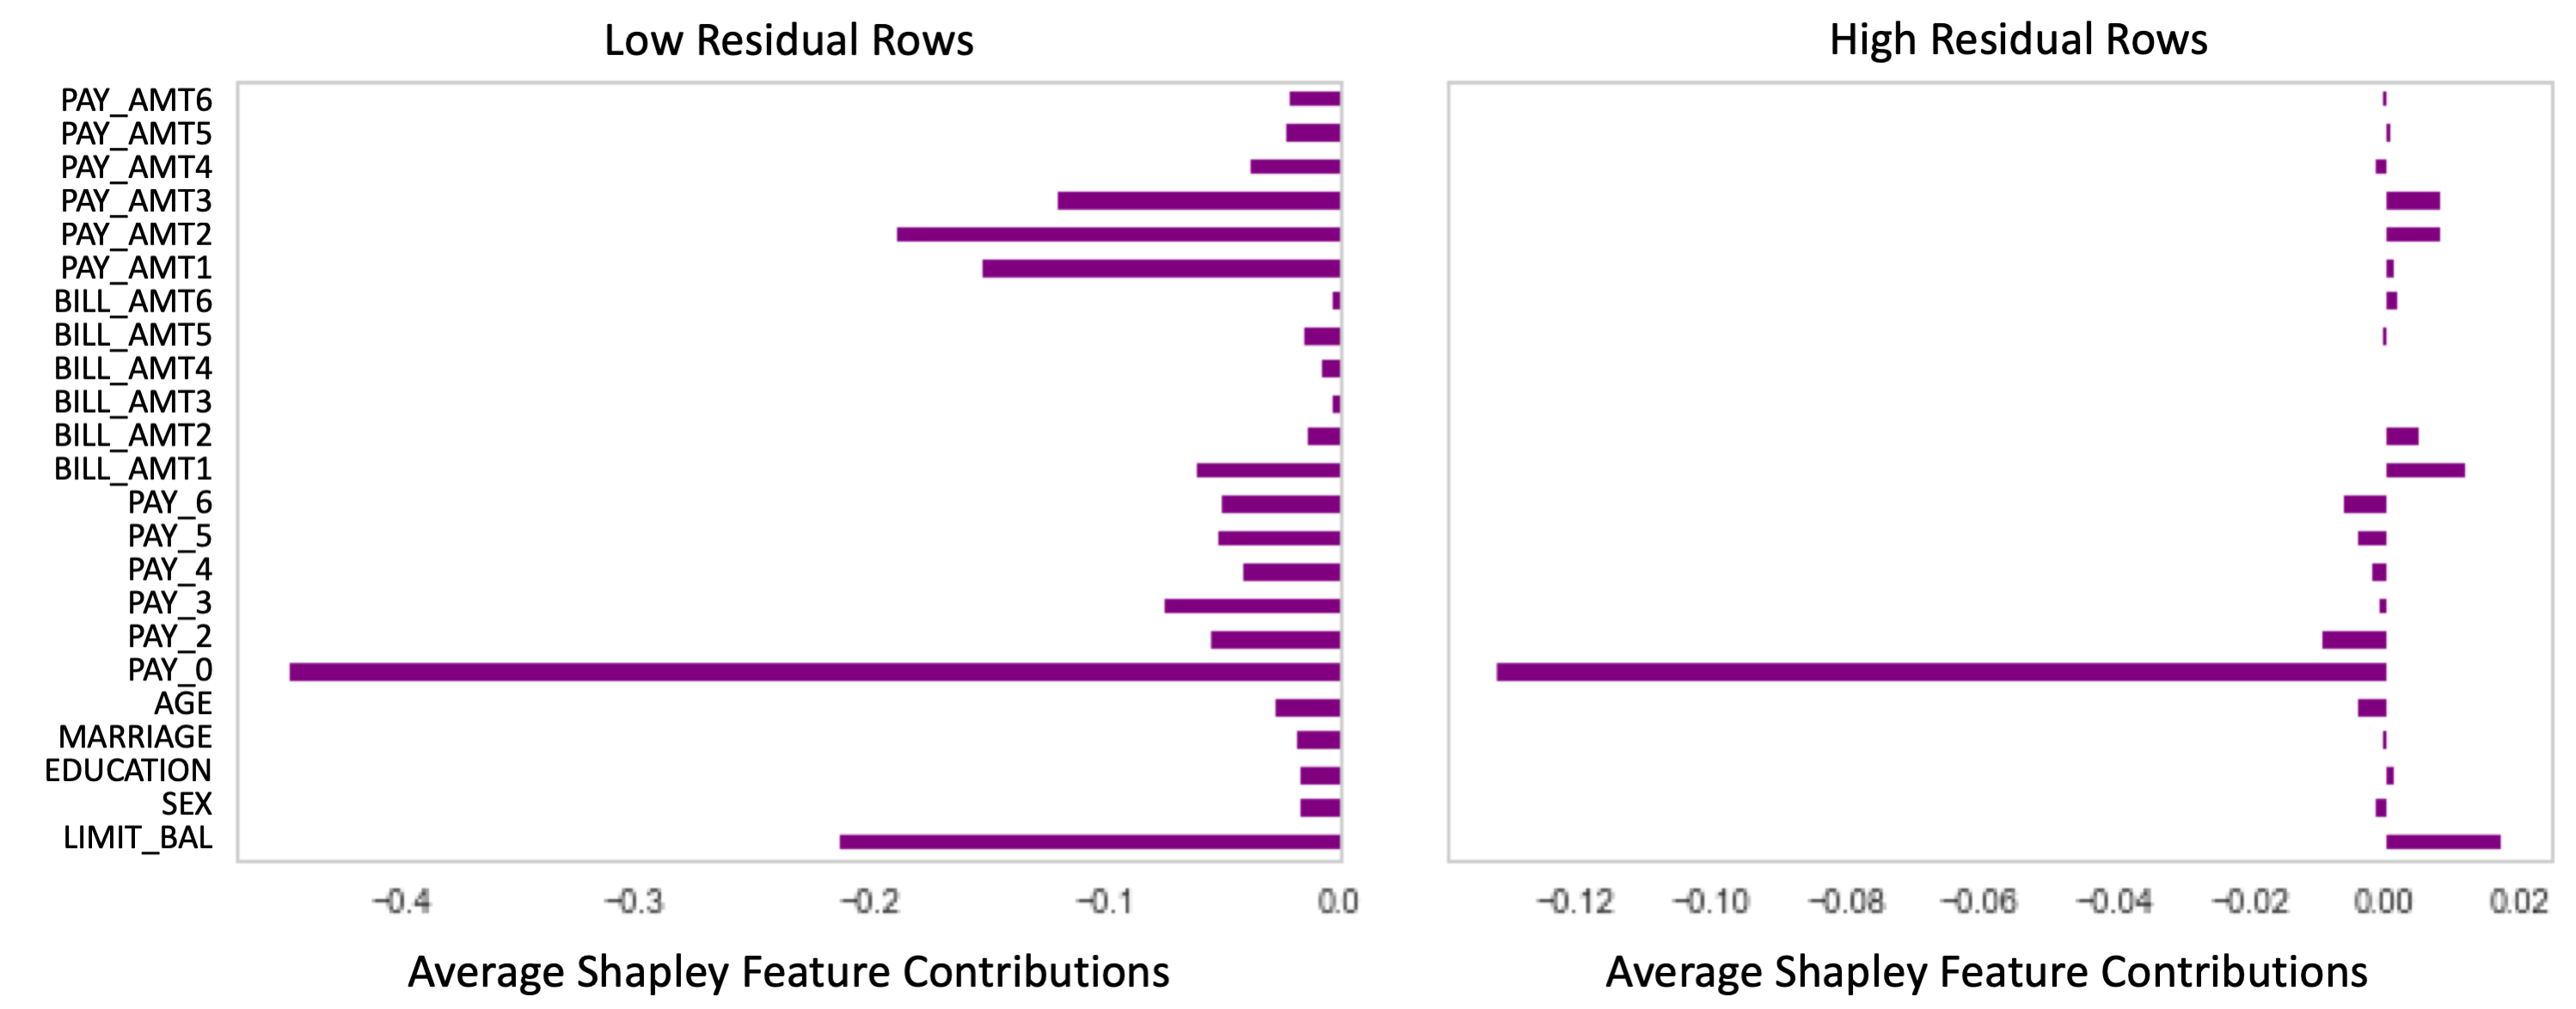
\includegraphics[height=125pt]{../img/global_high_low.png}
					\end{center}
				\end{figure}	
				\scriptsize{Exact local Shapley feature contributions \cite{shapley}, which are available at scoring time for unlabeled data, are noticeably different for low and high residual predictions. (Both monotonicity constraints and Shapley values are available in \href{https://www.github.com/h2oai/h2o-3}{h2o-3} and \href{https://www.github.com/dmlc/xgboost}{XGBoost}.)} 
		
			\end{frame}

			\begin{frame}[t]
		
				\frametitle{\large{\textbf{Residual Analysis}: Non-Robust Features}}
				\vspace{-10pt}
				\begin{figure}
					\begin{center}
						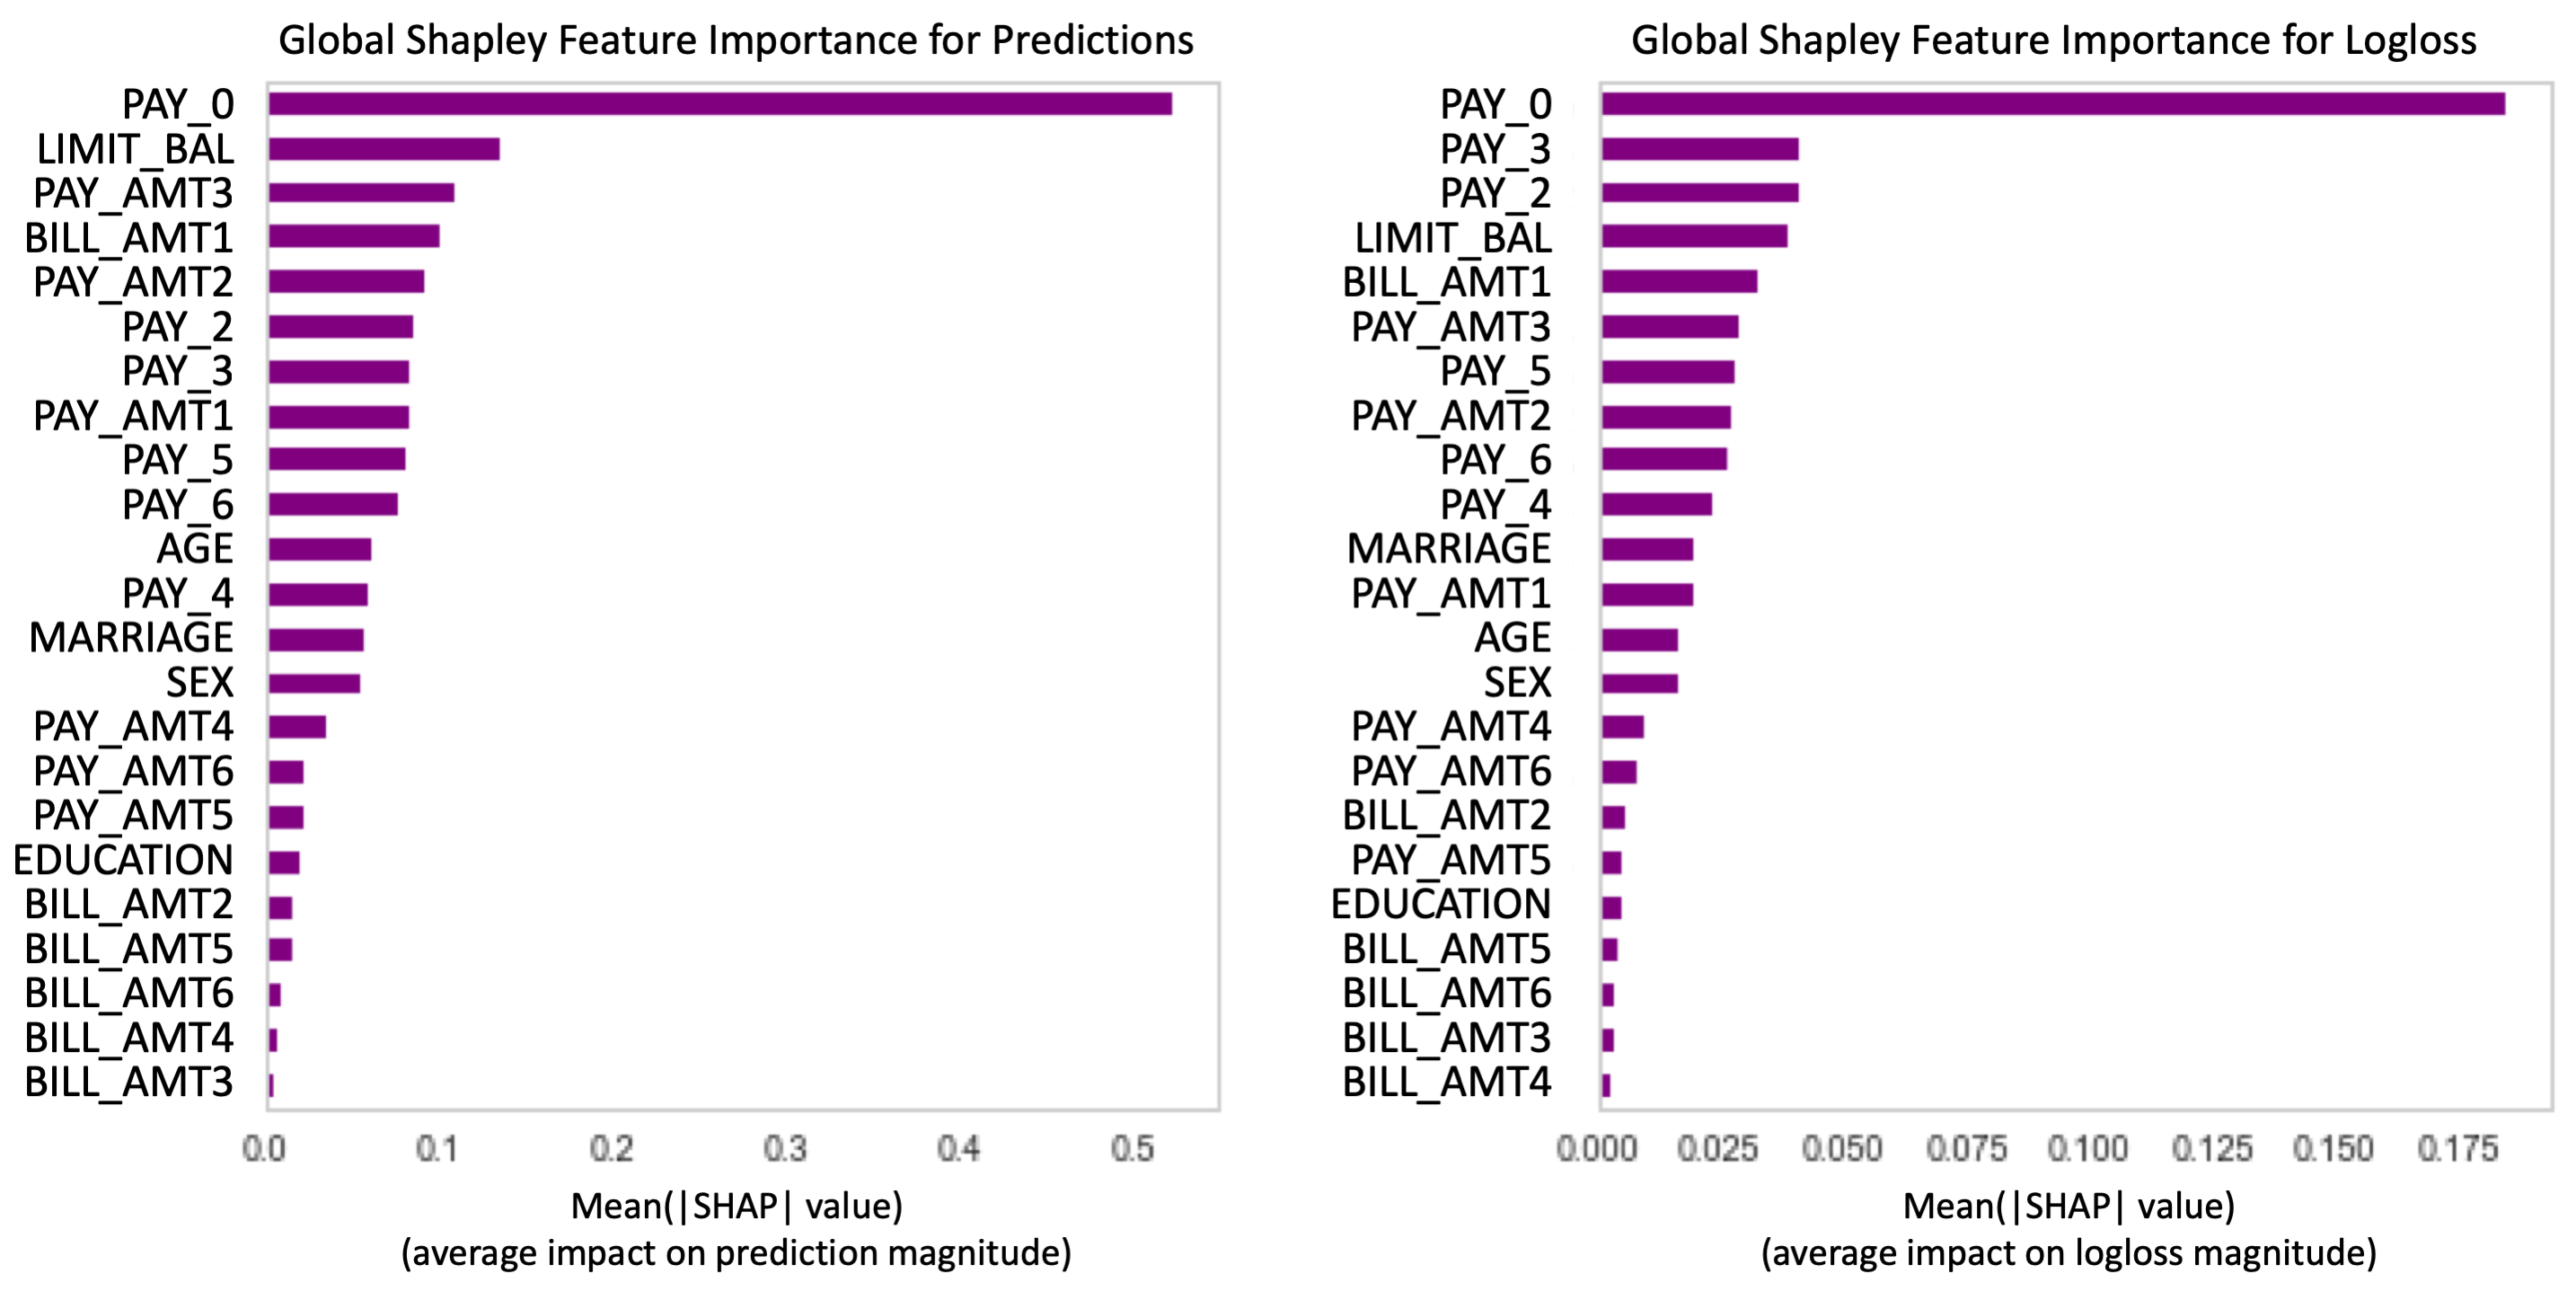
\includegraphics[height=150pt]{../img/global_pred_loss.png}
					\end{center}
				\end{figure}
				\vspace{-8pt}	
				\scriptsize{Globally important features $\text{PAY\_3}$ and $\text{PAY\_2}$ are more important, on average, to the loss than to the predictions. (Shapley contributions to XGBoost logloss can be calculated using the \href{https://github.com/slundberg/shap}{shap} package. This is a \textbf{time-consuming} calculation.)} 
		
			\end{frame}

			\begin{frame}
		
				\frametitle{\textbf{Residual Analysis}: Local Contributions to Logloss}
		
				\begin{figure}
					\begin{center}
						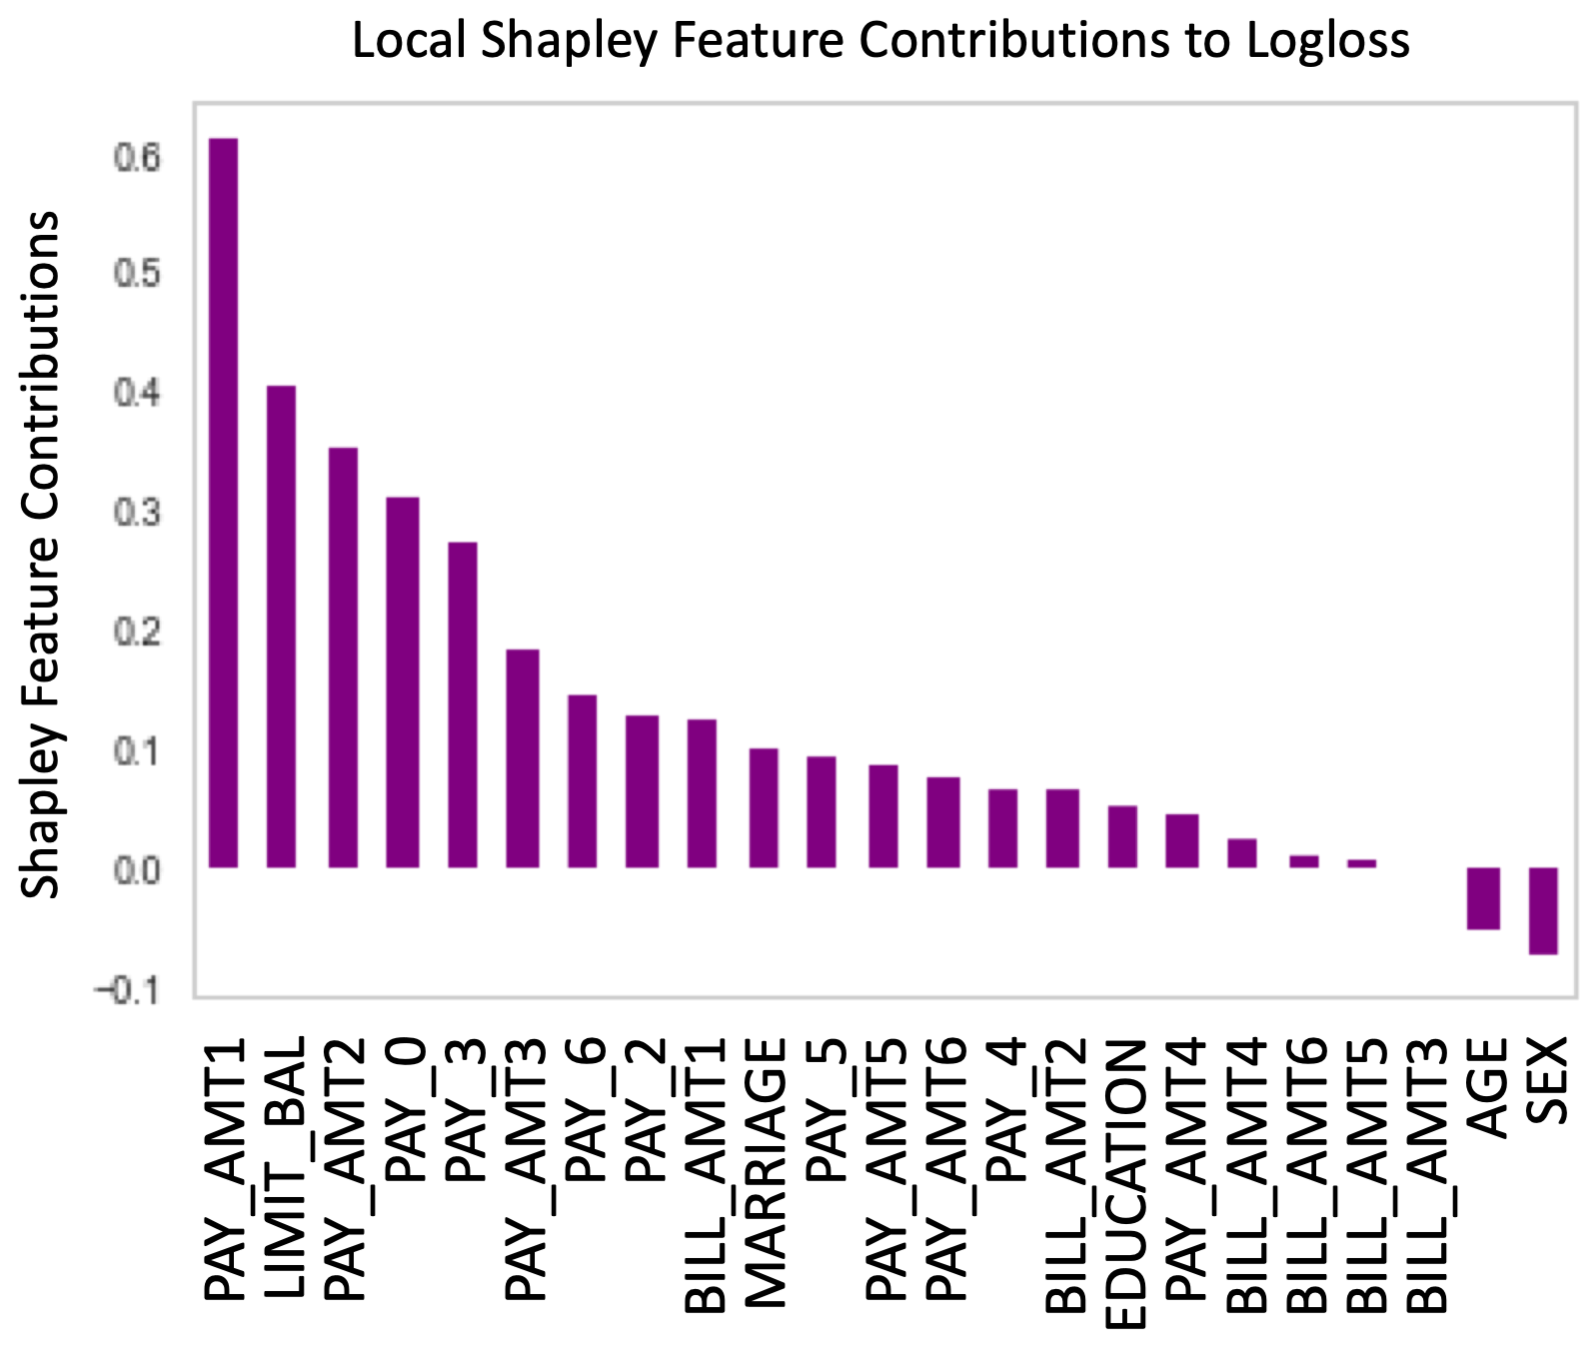
\includegraphics[height=130pt]{../img/local.png}
					\end{center}
				\end{figure}	
				Exact, local feature contributions to logloss can be calculated, enabling ranking of features contributing to logloss residuals for \textbf{each prediction}.
			\end{frame}

			\begin{frame}[t]
		
				\frametitle{\textbf{Residual Analysis}: Modeling Residuals}
				Decision tree model of $g_{\text{mono}} ~\text{DEFAULT\_NEXT\_MONTH} =1$ logloss residuals with 3-fold CV MSE $=0.0070$ and $R^2=0.8871$.
				\begin{figure}
					\begin{center}
						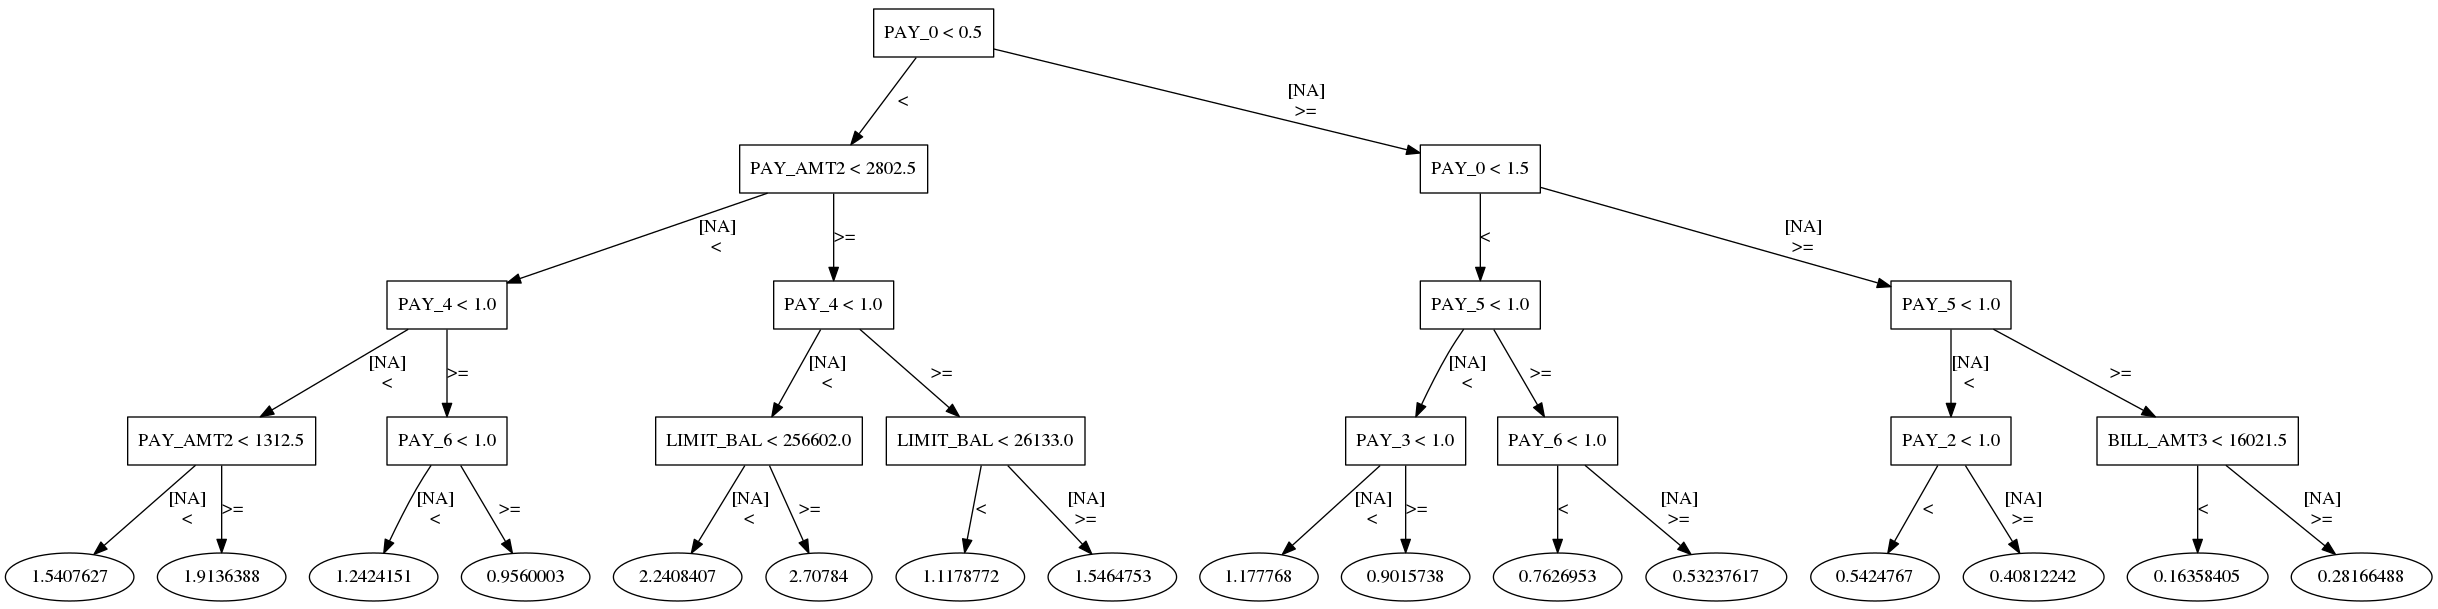
\includegraphics[height=95pt, width=330pt]{../img/surrogate_dt_1.png}
					\end{center}
				\end{figure}	
				This tree encodes rules describing when $g_{\text{mono}}$ is probably wrong.
			\end{frame}
			
%-------------------------------------------------------------------------------
		\subsection{Benchmark Models}
%-------------------------------------------------------------------------------	

			\begin{frame}
		
				\frametitle{\textbf{Benchmark Models}: Compare to Linear Models}
				\begin{figure}
					\begin{center}
						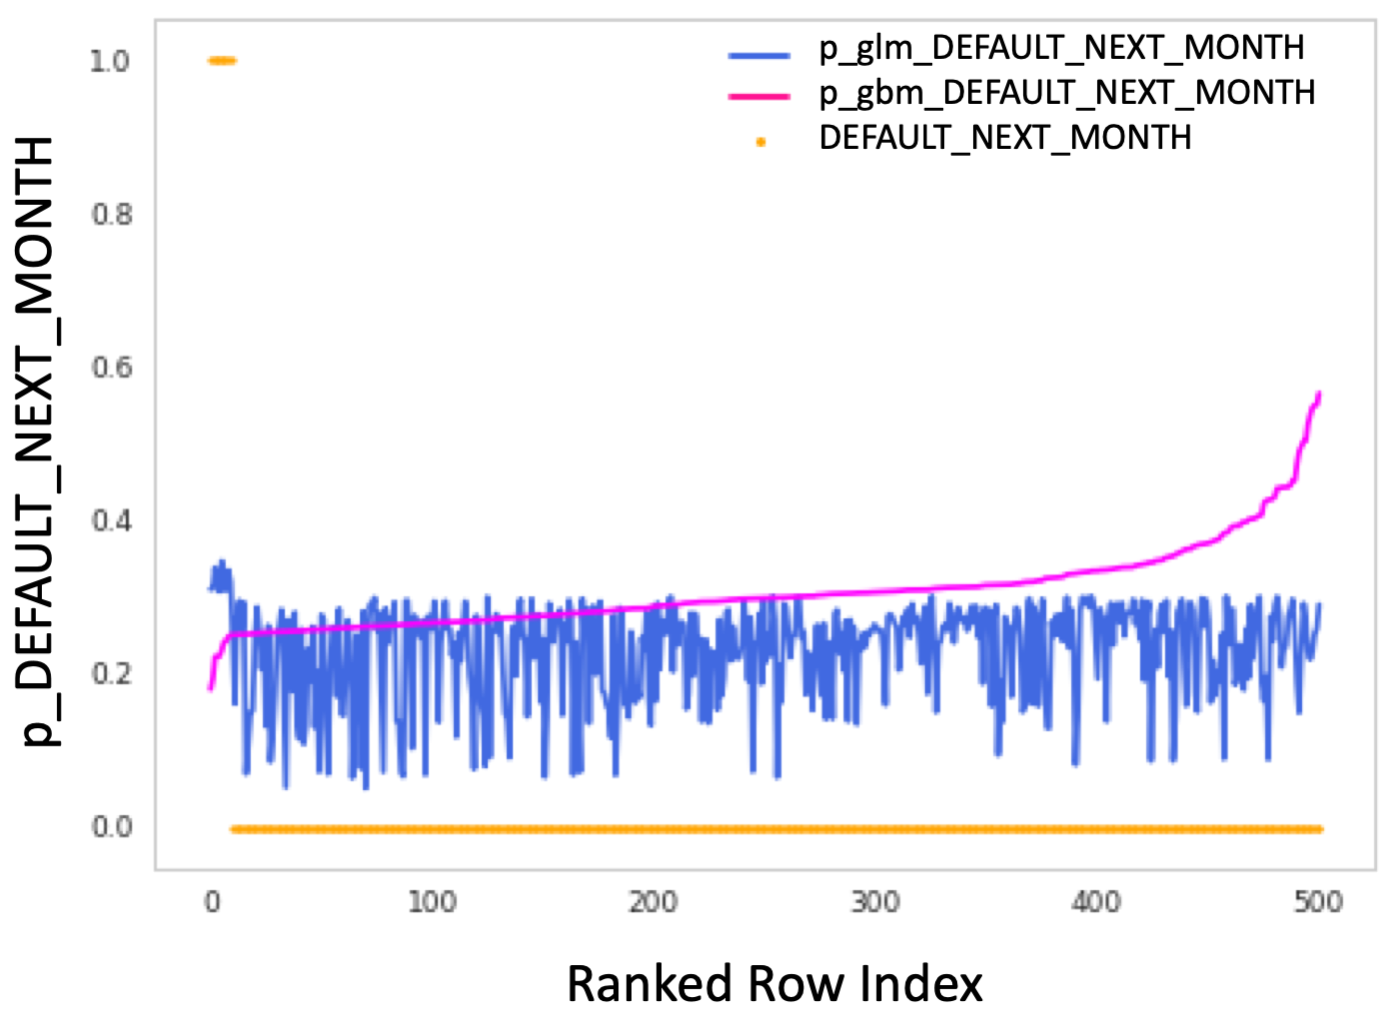
\includegraphics[height=130pt]{../img/benchmark.png}
					\end{center}
				\end{figure}	
				\vspace{-10pt}
				For a range of probabilities $\in  (\sim0.2, \sim0.6)$, $g_{\text{mono}}$ displays exactly incorrect prediction behavior as compared to a benchmark GLM.
			\end{frame}

%-------------------------------------------------------------------------------
		\subsection{Error Remediation}
%-------------------------------------------------------------------------------	

			\begin{frame}
		
				\frametitle{\textbf{Remediation}: for $g_{\text{mono}}$}
				
				\begin{itemize}\scriptsize
					\item \textbf{Over-emphasis of $\text{PAY\_0}$}:
					\begin{itemize}\scriptsize
						\item Engineer features for payment trends or stability.
						\item Missing value injection during training or scoring.
					\end{itemize}
					\item \textbf{Sparsity of $\text{PAY\_0} > 2$ training data}: Increase observation weights. 
					\item \textbf{Payments $\geq$ credit limit}: Scoring-time model assertion \cite{kangdebugging}. 
					\item \textbf{Disparate impact}: Adversarial de-biasing \cite{zhang2018mitigating} or model selection by minimal disparate impact. 
					\item \textbf{Security vulnerabilities}: API throttling, authentication, real-time model monitoring. 
					\item \textbf{Large logloss importance}: Evaluate dropping non-robust features.
					\item \textbf{Poor accuracy vs. benchmark GLM}: Blend $g_{\text{mono}}$ and GLM for probabilities $\in (\sim0.2, \sim0.6)$.
					\item \textbf{Miscellaneous strategies}: 
					\begin{itemize}\scriptsize
						\item Local feature importance and decision tree rules can indicate additional scoring-time model assertions, e.g. alternate treatment for locally non-robust features in known high-residual ranges of the learned response function. 
						\item Incorporate local feature contributions to logloss into training or scoring processes.
					\end{itemize}
				\end{itemize}
				\normalsize

			\end{frame}		
			
			\begin{frame}
		
				\frametitle{\textbf{Remediation}: General Strategies}

				\begin{itemize}
					\item Calibration to past data.
					\item Data collection or simulation for model blindspots.
					\item Detection and elimination of non-robust features.
					\item Missing value injection during training or scoring.
					\item Model or model artifact editing.
				\end{itemize}				
				
			\end{frame}



%-------------------------------------------------------------------------------
	\section{Acknowledgements} 
%-------------------------------------------------------------------------------

		\begin{frame}
			
			\frametitle{Acknowledgments}
			
				Thanks to Lisa Song for her continued assistance in developing these course materials.\\
				\vspace{10pt}
				Some materials \copyright\hspace{1pt}Patrick Hall and the H2O.ai team 2017-2020.  
			
		\end{frame}	

		\begin{frame}[t, allowframebreaks]
	
			\frametitle{References}	

			Advanced code examples for this presentation:\\
			\small{\url{https://www.github.com/jphall663/interpretable_machine_learning_with_python}}\\
			\noindent \small{\url{https://www.github.com/jphall663/responsible_xai}}
								
		\framebreak		
		
		\printbibliography
		
	\end{frame}

\end{document}